\documentclass{article}

    \usepackage[breakable]{tcolorbox}
    \usepackage{parskip} % Stop auto-indenting (to mimic markdown behaviour)
    

    % Basic figure setup, for now with no caption control since it's done
    % automatically by Pandoc (which extracts ![](path) syntax from Markdown).
    \usepackage{graphicx}
    % Maintain compatibility with old templates. Remove in nbconvert 6.0
    \let\Oldincludegraphics\includegraphics
    % Ensure that by default, figures have no caption (until we provide a
    % proper Figure object with a Caption API and a way to capture that
    % in the conversion process - todo).
    \usepackage{caption}
    \DeclareCaptionFormat{nocaption}{}
    \captionsetup{format=nocaption,aboveskip=0pt,belowskip=0pt}

    \usepackage{float}
    \floatplacement{figure}{H} % forces figures to be placed at the correct location
    \usepackage{xcolor} % Allow colors to be defined
    \usepackage{enumerate} % Needed for markdown enumerations to work
    \usepackage{geometry} % Used to adjust the document margins
    \usepackage{amsmath} % Equations
    \usepackage{amssymb} % Equations
    \usepackage{textcomp} % defines textquotesingle
    % Hack from http://tex.stackexchange.com/a/47451/13684:
    \AtBeginDocument{%
        \def\PYZsq{\textquotesingle}% Upright quotes in Pygmentized code
    }
    \usepackage{upquote} % Upright quotes for verbatim code
    \usepackage{eurosym} % defines \euro

    \usepackage{iftex}
    \ifPDFTeX
        \usepackage[T1]{fontenc}
        \IfFileExists{alphabeta.sty}{
              \usepackage{alphabeta}
          }{
              \usepackage[mathletters]{ucs}
              \usepackage[utf8x]{inputenc}
          }
    \else
        \usepackage{fontspec}
        \usepackage{unicode-math}
    \fi

    \usepackage{fancyvrb} % verbatim replacement that allows latex
    \usepackage{grffile} % extends the file name processing of package graphics
                         % to support a larger range
    \makeatletter % fix for old versions of grffile with XeLaTeX
    \@ifpackagelater{grffile}{2019/11/01}
    {
      % Do nothing on new versions
    }
    {
      \def\Gread@@xetex#1{%
        \IfFileExists{"\Gin@base".bb}%
        {\Gread@eps{\Gin@base.bb}}%
        {\Gread@@xetex@aux#1}%
      }
    }
    \makeatother
    \usepackage[Export]{adjustbox} % Used to constrain images to a maximum size
    \adjustboxset{max size={0.9\linewidth}{0.9\paperheight}}

    % The hyperref package gives us a pdf with properly built
    % internal navigation ('pdf bookmarks' for the table of contents,
    % internal cross-reference links, web links for URLs, etc.)
    \usepackage{hyperref}
    % The default LaTeX title has an obnoxious amount of whitespace. By default,
    % titling removes some of it. It also provides customization options.
    \usepackage{titling}
    \usepackage{longtable} % longtable support required by pandoc >1.10
    \usepackage{booktabs}  % table support for pandoc > 1.12.2
    \usepackage{array}     % table support for pandoc >= 2.11.3
    \usepackage{calc}      % table minipage width calculation for pandoc >= 2.11.1
    \usepackage[inline]{enumitem} % IRkernel/repr support (it uses the enumerate* environment)
    \usepackage[normalem]{ulem} % ulem is needed to support strikethroughs (\sout)
                                % normalem makes italics be italics, not underlines
    \usepackage{mathrsfs}
    

    
    % Colors for the hyperref package
    \definecolor{urlcolor}{rgb}{0,.145,.698}
    \definecolor{linkcolor}{rgb}{.71,0.21,0.01}
    \definecolor{citecolor}{rgb}{.12,.54,.11}

    % ANSI colors
    \definecolor{ansi-black}{HTML}{3E424D}
    \definecolor{ansi-black-intense}{HTML}{282C36}
    \definecolor{ansi-red}{HTML}{E75C58}
    \definecolor{ansi-red-intense}{HTML}{B22B31}
    \definecolor{ansi-green}{HTML}{00A250}
    \definecolor{ansi-green-intense}{HTML}{007427}
    \definecolor{ansi-yellow}{HTML}{DDB62B}
    \definecolor{ansi-yellow-intense}{HTML}{B27D12}
    \definecolor{ansi-blue}{HTML}{208FFB}
    \definecolor{ansi-blue-intense}{HTML}{0065CA}
    \definecolor{ansi-magenta}{HTML}{D160C4}
    \definecolor{ansi-magenta-intense}{HTML}{A03196}
    \definecolor{ansi-cyan}{HTML}{60C6C8}
    \definecolor{ansi-cyan-intense}{HTML}{258F8F}
    \definecolor{ansi-white}{HTML}{C5C1B4}
    \definecolor{ansi-white-intense}{HTML}{A1A6B2}
    \definecolor{ansi-default-inverse-fg}{HTML}{FFFFFF}
    \definecolor{ansi-default-inverse-bg}{HTML}{000000}

    % common color for the border for error outputs.
    \definecolor{outerrorbackground}{HTML}{FFDFDF}

    % commands and environments needed by pandoc snippets
    % extracted from the output of `pandoc -s`
    \providecommand{\tightlist}{%
      \setlength{\itemsep}{0pt}\setlength{\parskip}{0pt}}
    \DefineVerbatimEnvironment{Highlighting}{Verbatim}{commandchars=\\\{\}}
    % Add ',fontsize=\small' for more characters per line
    \newenvironment{Shaded}{}{}
    \newcommand{\KeywordTok}[1]{\textcolor[rgb]{0.00,0.44,0.13}{\textbf{{#1}}}}
    \newcommand{\DataTypeTok}[1]{\textcolor[rgb]{0.56,0.13,0.00}{{#1}}}
    \newcommand{\DecValTok}[1]{\textcolor[rgb]{0.25,0.63,0.44}{{#1}}}
    \newcommand{\BaseNTok}[1]{\textcolor[rgb]{0.25,0.63,0.44}{{#1}}}
    \newcommand{\FloatTok}[1]{\textcolor[rgb]{0.25,0.63,0.44}{{#1}}}
    \newcommand{\CharTok}[1]{\textcolor[rgb]{0.25,0.44,0.63}{{#1}}}
    \newcommand{\StringTok}[1]{\textcolor[rgb]{0.25,0.44,0.63}{{#1}}}
    \newcommand{\CommentTok}[1]{\textcolor[rgb]{0.38,0.63,0.69}{\textit{{#1}}}}
    \newcommand{\OtherTok}[1]{\textcolor[rgb]{0.00,0.44,0.13}{{#1}}}
    \newcommand{\AlertTok}[1]{\textcolor[rgb]{1.00,0.00,0.00}{\textbf{{#1}}}}
    \newcommand{\FunctionTok}[1]{\textcolor[rgb]{0.02,0.16,0.49}{{#1}}}
    \newcommand{\RegionMarkerTok}[1]{{#1}}
    \newcommand{\ErrorTok}[1]{\textcolor[rgb]{1.00,0.00,0.00}{\textbf{{#1}}}}
    \newcommand{\NormalTok}[1]{{#1}}

    % Additional commands for more recent versions of Pandoc
    \newcommand{\ConstantTok}[1]{\textcolor[rgb]{0.53,0.00,0.00}{{#1}}}
    \newcommand{\SpecialCharTok}[1]{\textcolor[rgb]{0.25,0.44,0.63}{{#1}}}
    \newcommand{\VerbatimStringTok}[1]{\textcolor[rgb]{0.25,0.44,0.63}{{#1}}}
    \newcommand{\SpecialStringTok}[1]{\textcolor[rgb]{0.73,0.40,0.53}{{#1}}}
    \newcommand{\ImportTok}[1]{{#1}}
    \newcommand{\DocumentationTok}[1]{\textcolor[rgb]{0.73,0.13,0.13}{\textit{{#1}}}}
    \newcommand{\AnnotationTok}[1]{\textcolor[rgb]{0.38,0.63,0.69}{\textbf{\textit{{#1}}}}}
    \newcommand{\CommentVarTok}[1]{\textcolor[rgb]{0.38,0.63,0.69}{\textbf{\textit{{#1}}}}}
    \newcommand{\VariableTok}[1]{\textcolor[rgb]{0.10,0.09,0.49}{{#1}}}
    \newcommand{\ControlFlowTok}[1]{\textcolor[rgb]{0.00,0.44,0.13}{\textbf{{#1}}}}
    \newcommand{\OperatorTok}[1]{\textcolor[rgb]{0.40,0.40,0.40}{{#1}}}
    \newcommand{\BuiltInTok}[1]{{#1}}
    \newcommand{\ExtensionTok}[1]{{#1}}
    \newcommand{\PreprocessorTok}[1]{\textcolor[rgb]{0.74,0.48,0.00}{{#1}}}
    \newcommand{\AttributeTok}[1]{\textcolor[rgb]{0.49,0.56,0.16}{{#1}}}
    \newcommand{\InformationTok}[1]{\textcolor[rgb]{0.38,0.63,0.69}{\textbf{\textit{{#1}}}}}
    \newcommand{\WarningTok}[1]{\textcolor[rgb]{0.38,0.63,0.69}{\textbf{\textit{{#1}}}}}


    % Define a nice break command that doesn't care if a line doesn't already
    % exist.
    \def\br{\hspace*{\fill} \\* }
    % Math Jax compatibility definitions
    \def\gt{>}
    \def\lt{<}
    \let\Oldtex\TeX
    \let\Oldlatex\LaTeX
    \renewcommand{\TeX}{\textrm{\Oldtex}}
    \renewcommand{\LaTeX}{\textrm{\Oldlatex}}
    % Document parameters
    % Document title
    \title{fourier}
    
    
    
    
    
    
    
% Pygments definitions
\makeatletter
\def\PY@reset{\let\PY@it=\relax \let\PY@bf=\relax%
    \let\PY@ul=\relax \let\PY@tc=\relax%
    \let\PY@bc=\relax \let\PY@ff=\relax}
\def\PY@tok#1{\csname PY@tok@#1\endcsname}
\def\PY@toks#1+{\ifx\relax#1\empty\else%
    \PY@tok{#1}\expandafter\PY@toks\fi}
\def\PY@do#1{\PY@bc{\PY@tc{\PY@ul{%
    \PY@it{\PY@bf{\PY@ff{#1}}}}}}}
\def\PY#1#2{\PY@reset\PY@toks#1+\relax+\PY@do{#2}}

\@namedef{PY@tok@w}{\def\PY@tc##1{\textcolor[rgb]{0.73,0.73,0.73}{##1}}}
\@namedef{PY@tok@c}{\let\PY@it=\textit\def\PY@tc##1{\textcolor[rgb]{0.24,0.48,0.48}{##1}}}
\@namedef{PY@tok@cp}{\def\PY@tc##1{\textcolor[rgb]{0.61,0.40,0.00}{##1}}}
\@namedef{PY@tok@k}{\let\PY@bf=\textbf\def\PY@tc##1{\textcolor[rgb]{0.00,0.50,0.00}{##1}}}
\@namedef{PY@tok@kp}{\def\PY@tc##1{\textcolor[rgb]{0.00,0.50,0.00}{##1}}}
\@namedef{PY@tok@kt}{\def\PY@tc##1{\textcolor[rgb]{0.69,0.00,0.25}{##1}}}
\@namedef{PY@tok@o}{\def\PY@tc##1{\textcolor[rgb]{0.40,0.40,0.40}{##1}}}
\@namedef{PY@tok@ow}{\let\PY@bf=\textbf\def\PY@tc##1{\textcolor[rgb]{0.67,0.13,1.00}{##1}}}
\@namedef{PY@tok@nb}{\def\PY@tc##1{\textcolor[rgb]{0.00,0.50,0.00}{##1}}}
\@namedef{PY@tok@nf}{\def\PY@tc##1{\textcolor[rgb]{0.00,0.00,1.00}{##1}}}
\@namedef{PY@tok@nc}{\let\PY@bf=\textbf\def\PY@tc##1{\textcolor[rgb]{0.00,0.00,1.00}{##1}}}
\@namedef{PY@tok@nn}{\let\PY@bf=\textbf\def\PY@tc##1{\textcolor[rgb]{0.00,0.00,1.00}{##1}}}
\@namedef{PY@tok@ne}{\let\PY@bf=\textbf\def\PY@tc##1{\textcolor[rgb]{0.80,0.25,0.22}{##1}}}
\@namedef{PY@tok@nv}{\def\PY@tc##1{\textcolor[rgb]{0.10,0.09,0.49}{##1}}}
\@namedef{PY@tok@no}{\def\PY@tc##1{\textcolor[rgb]{0.53,0.00,0.00}{##1}}}
\@namedef{PY@tok@nl}{\def\PY@tc##1{\textcolor[rgb]{0.46,0.46,0.00}{##1}}}
\@namedef{PY@tok@ni}{\let\PY@bf=\textbf\def\PY@tc##1{\textcolor[rgb]{0.44,0.44,0.44}{##1}}}
\@namedef{PY@tok@na}{\def\PY@tc##1{\textcolor[rgb]{0.41,0.47,0.13}{##1}}}
\@namedef{PY@tok@nt}{\let\PY@bf=\textbf\def\PY@tc##1{\textcolor[rgb]{0.00,0.50,0.00}{##1}}}
\@namedef{PY@tok@nd}{\def\PY@tc##1{\textcolor[rgb]{0.67,0.13,1.00}{##1}}}
\@namedef{PY@tok@s}{\def\PY@tc##1{\textcolor[rgb]{0.73,0.13,0.13}{##1}}}
\@namedef{PY@tok@sd}{\let\PY@it=\textit\def\PY@tc##1{\textcolor[rgb]{0.73,0.13,0.13}{##1}}}
\@namedef{PY@tok@si}{\let\PY@bf=\textbf\def\PY@tc##1{\textcolor[rgb]{0.64,0.35,0.47}{##1}}}
\@namedef{PY@tok@se}{\let\PY@bf=\textbf\def\PY@tc##1{\textcolor[rgb]{0.67,0.36,0.12}{##1}}}
\@namedef{PY@tok@sr}{\def\PY@tc##1{\textcolor[rgb]{0.64,0.35,0.47}{##1}}}
\@namedef{PY@tok@ss}{\def\PY@tc##1{\textcolor[rgb]{0.10,0.09,0.49}{##1}}}
\@namedef{PY@tok@sx}{\def\PY@tc##1{\textcolor[rgb]{0.00,0.50,0.00}{##1}}}
\@namedef{PY@tok@m}{\def\PY@tc##1{\textcolor[rgb]{0.40,0.40,0.40}{##1}}}
\@namedef{PY@tok@gh}{\let\PY@bf=\textbf\def\PY@tc##1{\textcolor[rgb]{0.00,0.00,0.50}{##1}}}
\@namedef{PY@tok@gu}{\let\PY@bf=\textbf\def\PY@tc##1{\textcolor[rgb]{0.50,0.00,0.50}{##1}}}
\@namedef{PY@tok@gd}{\def\PY@tc##1{\textcolor[rgb]{0.63,0.00,0.00}{##1}}}
\@namedef{PY@tok@gi}{\def\PY@tc##1{\textcolor[rgb]{0.00,0.52,0.00}{##1}}}
\@namedef{PY@tok@gr}{\def\PY@tc##1{\textcolor[rgb]{0.89,0.00,0.00}{##1}}}
\@namedef{PY@tok@ge}{\let\PY@it=\textit}
\@namedef{PY@tok@gs}{\let\PY@bf=\textbf}
\@namedef{PY@tok@gp}{\let\PY@bf=\textbf\def\PY@tc##1{\textcolor[rgb]{0.00,0.00,0.50}{##1}}}
\@namedef{PY@tok@go}{\def\PY@tc##1{\textcolor[rgb]{0.44,0.44,0.44}{##1}}}
\@namedef{PY@tok@gt}{\def\PY@tc##1{\textcolor[rgb]{0.00,0.27,0.87}{##1}}}
\@namedef{PY@tok@err}{\def\PY@bc##1{{\setlength{\fboxsep}{\string -\fboxrule}\fcolorbox[rgb]{1.00,0.00,0.00}{1,1,1}{\strut ##1}}}}
\@namedef{PY@tok@kc}{\let\PY@bf=\textbf\def\PY@tc##1{\textcolor[rgb]{0.00,0.50,0.00}{##1}}}
\@namedef{PY@tok@kd}{\let\PY@bf=\textbf\def\PY@tc##1{\textcolor[rgb]{0.00,0.50,0.00}{##1}}}
\@namedef{PY@tok@kn}{\let\PY@bf=\textbf\def\PY@tc##1{\textcolor[rgb]{0.00,0.50,0.00}{##1}}}
\@namedef{PY@tok@kr}{\let\PY@bf=\textbf\def\PY@tc##1{\textcolor[rgb]{0.00,0.50,0.00}{##1}}}
\@namedef{PY@tok@bp}{\def\PY@tc##1{\textcolor[rgb]{0.00,0.50,0.00}{##1}}}
\@namedef{PY@tok@fm}{\def\PY@tc##1{\textcolor[rgb]{0.00,0.00,1.00}{##1}}}
\@namedef{PY@tok@vc}{\def\PY@tc##1{\textcolor[rgb]{0.10,0.09,0.49}{##1}}}
\@namedef{PY@tok@vg}{\def\PY@tc##1{\textcolor[rgb]{0.10,0.09,0.49}{##1}}}
\@namedef{PY@tok@vi}{\def\PY@tc##1{\textcolor[rgb]{0.10,0.09,0.49}{##1}}}
\@namedef{PY@tok@vm}{\def\PY@tc##1{\textcolor[rgb]{0.10,0.09,0.49}{##1}}}
\@namedef{PY@tok@sa}{\def\PY@tc##1{\textcolor[rgb]{0.73,0.13,0.13}{##1}}}
\@namedef{PY@tok@sb}{\def\PY@tc##1{\textcolor[rgb]{0.73,0.13,0.13}{##1}}}
\@namedef{PY@tok@sc}{\def\PY@tc##1{\textcolor[rgb]{0.73,0.13,0.13}{##1}}}
\@namedef{PY@tok@dl}{\def\PY@tc##1{\textcolor[rgb]{0.73,0.13,0.13}{##1}}}
\@namedef{PY@tok@s2}{\def\PY@tc##1{\textcolor[rgb]{0.73,0.13,0.13}{##1}}}
\@namedef{PY@tok@sh}{\def\PY@tc##1{\textcolor[rgb]{0.73,0.13,0.13}{##1}}}
\@namedef{PY@tok@s1}{\def\PY@tc##1{\textcolor[rgb]{0.73,0.13,0.13}{##1}}}
\@namedef{PY@tok@mb}{\def\PY@tc##1{\textcolor[rgb]{0.40,0.40,0.40}{##1}}}
\@namedef{PY@tok@mf}{\def\PY@tc##1{\textcolor[rgb]{0.40,0.40,0.40}{##1}}}
\@namedef{PY@tok@mh}{\def\PY@tc##1{\textcolor[rgb]{0.40,0.40,0.40}{##1}}}
\@namedef{PY@tok@mi}{\def\PY@tc##1{\textcolor[rgb]{0.40,0.40,0.40}{##1}}}
\@namedef{PY@tok@il}{\def\PY@tc##1{\textcolor[rgb]{0.40,0.40,0.40}{##1}}}
\@namedef{PY@tok@mo}{\def\PY@tc##1{\textcolor[rgb]{0.40,0.40,0.40}{##1}}}
\@namedef{PY@tok@ch}{\let\PY@it=\textit\def\PY@tc##1{\textcolor[rgb]{0.24,0.48,0.48}{##1}}}
\@namedef{PY@tok@cm}{\let\PY@it=\textit\def\PY@tc##1{\textcolor[rgb]{0.24,0.48,0.48}{##1}}}
\@namedef{PY@tok@cpf}{\let\PY@it=\textit\def\PY@tc##1{\textcolor[rgb]{0.24,0.48,0.48}{##1}}}
\@namedef{PY@tok@c1}{\let\PY@it=\textit\def\PY@tc##1{\textcolor[rgb]{0.24,0.48,0.48}{##1}}}
\@namedef{PY@tok@cs}{\let\PY@it=\textit\def\PY@tc##1{\textcolor[rgb]{0.24,0.48,0.48}{##1}}}

\def\PYZbs{\char`\\}
\def\PYZus{\char`\_}
\def\PYZob{\char`\{}
\def\PYZcb{\char`\}}
\def\PYZca{\char`\^}
\def\PYZam{\char`\&}
\def\PYZlt{\char`\<}
\def\PYZgt{\char`\>}
\def\PYZsh{\char`\#}
\def\PYZpc{\char`\%}
\def\PYZdl{\char`\$}
\def\PYZhy{\char`\-}
\def\PYZsq{\char`\'}
\def\PYZdq{\char`\"}
\def\PYZti{\char`\~}
% for compatibility with earlier versions
\def\PYZat{@}
\def\PYZlb{[}
\def\PYZrb{]}
\makeatother


    % For linebreaks inside Verbatim environment from package fancyvrb.
    \makeatletter
        \newbox\Wrappedcontinuationbox
        \newbox\Wrappedvisiblespacebox
        \newcommand*\Wrappedvisiblespace {\textcolor{red}{\textvisiblespace}}
        \newcommand*\Wrappedcontinuationsymbol {\textcolor{red}{\llap{\tiny$\m@th\hookrightarrow$}}}
        \newcommand*\Wrappedcontinuationindent {3ex }
        \newcommand*\Wrappedafterbreak {\kern\Wrappedcontinuationindent\copy\Wrappedcontinuationbox}
        % Take advantage of the already applied Pygments mark-up to insert
        % potential linebreaks for TeX processing.
        %        {, <, #, %, $, ' and ": go to next line.
        %        _, }, ^, &, >, - and ~: stay at end of broken line.
        % Use of \textquotesingle for straight quote.
        \newcommand*\Wrappedbreaksatspecials {%
            \def\PYGZus{\discretionary{\char`\_}{\Wrappedafterbreak}{\char`\_}}%
            \def\PYGZob{\discretionary{}{\Wrappedafterbreak\char`\{}{\char`\{}}%
            \def\PYGZcb{\discretionary{\char`\}}{\Wrappedafterbreak}{\char`\}}}%
            \def\PYGZca{\discretionary{\char`\^}{\Wrappedafterbreak}{\char`\^}}%
            \def\PYGZam{\discretionary{\char`\&}{\Wrappedafterbreak}{\char`\&}}%
            \def\PYGZlt{\discretionary{}{\Wrappedafterbreak\char`\<}{\char`\<}}%
            \def\PYGZgt{\discretionary{\char`\>}{\Wrappedafterbreak}{\char`\>}}%
            \def\PYGZsh{\discretionary{}{\Wrappedafterbreak\char`\#}{\char`\#}}%
            \def\PYGZpc{\discretionary{}{\Wrappedafterbreak\char`\%}{\char`\%}}%
            \def\PYGZdl{\discretionary{}{\Wrappedafterbreak\char`\$}{\char`\$}}%
            \def\PYGZhy{\discretionary{\char`\-}{\Wrappedafterbreak}{\char`\-}}%
            \def\PYGZsq{\discretionary{}{\Wrappedafterbreak\textquotesingle}{\textquotesingle}}%
            \def\PYGZdq{\discretionary{}{\Wrappedafterbreak\char`\"}{\char`\"}}%
            \def\PYGZti{\discretionary{\char`\~}{\Wrappedafterbreak}{\char`\~}}%
        }
        % Some characters . , ; ? ! / are not pygmentized.
        % This macro makes them "active" and they will insert potential linebreaks
        \newcommand*\Wrappedbreaksatpunct {%
            \lccode`\~`\.\lowercase{\def~}{\discretionary{\hbox{\char`\.}}{\Wrappedafterbreak}{\hbox{\char`\.}}}%
            \lccode`\~`\,\lowercase{\def~}{\discretionary{\hbox{\char`\,}}{\Wrappedafterbreak}{\hbox{\char`\,}}}%
            \lccode`\~`\;\lowercase{\def~}{\discretionary{\hbox{\char`\;}}{\Wrappedafterbreak}{\hbox{\char`\;}}}%
            \lccode`\~`\:\lowercase{\def~}{\discretionary{\hbox{\char`\:}}{\Wrappedafterbreak}{\hbox{\char`\:}}}%
            \lccode`\~`\?\lowercase{\def~}{\discretionary{\hbox{\char`\?}}{\Wrappedafterbreak}{\hbox{\char`\?}}}%
            \lccode`\~`\!\lowercase{\def~}{\discretionary{\hbox{\char`\!}}{\Wrappedafterbreak}{\hbox{\char`\!}}}%
            \lccode`\~`\/\lowercase{\def~}{\discretionary{\hbox{\char`\/}}{\Wrappedafterbreak}{\hbox{\char`\/}}}%
            \catcode`\.\active
            \catcode`\,\active
            \catcode`\;\active
            \catcode`\:\active
            \catcode`\?\active
            \catcode`\!\active
            \catcode`\/\active
            \lccode`\~`\~
        }
    \makeatother

    \let\OriginalVerbatim=\Verbatim
    \makeatletter
    \renewcommand{\Verbatim}[1][1]{%
        %\parskip\z@skip
        \sbox\Wrappedcontinuationbox {\Wrappedcontinuationsymbol}%
        \sbox\Wrappedvisiblespacebox {\FV@SetupFont\Wrappedvisiblespace}%
        \def\FancyVerbFormatLine ##1{\hsize\linewidth
            \vtop{\raggedright\hyphenpenalty\z@\exhyphenpenalty\z@
                \doublehyphendemerits\z@\finalhyphendemerits\z@
                \strut ##1\strut}%
        }%
        % If the linebreak is at a space, the latter will be displayed as visible
        % space at end of first line, and a continuation symbol starts next line.
        % Stretch/shrink are however usually zero for typewriter font.
        \def\FV@Space {%
            \nobreak\hskip\z@ plus\fontdimen3\font minus\fontdimen4\font
            \discretionary{\copy\Wrappedvisiblespacebox}{\Wrappedafterbreak}
            {\kern\fontdimen2\font}%
        }%

        % Allow breaks at special characters using \PYG... macros.
        \Wrappedbreaksatspecials
        % Breaks at punctuation characters . , ; ? ! and / need catcode=\active
        \OriginalVerbatim[#1,codes*=\Wrappedbreaksatpunct]%
    }
    \makeatother

    % Exact colors from NB
    \definecolor{incolor}{HTML}{303F9F}
    \definecolor{outcolor}{HTML}{D84315}
    \definecolor{cellborder}{HTML}{CFCFCF}
    \definecolor{cellbackground}{HTML}{F7F7F7}

    % prompt
    \makeatletter
    \newcommand{\boxspacing}{\kern\kvtcb@left@rule\kern\kvtcb@boxsep}
    \makeatother
    \newcommand{\prompt}[4]{
        {\ttfamily\llap{{\color{#2}[#3]:\hspace{3pt}#4}}\vspace{-\baselineskip}}
    }
    

    
    % Prevent overflowing lines due to hard-to-break entities
    \sloppy
    % Setup hyperref package
    \hypersetup{
      breaklinks=true,  % so long urls are correctly broken across lines
      colorlinks=true,
      urlcolor=urlcolor,
      linkcolor=linkcolor,
      citecolor=citecolor,
      }
    % Slightly bigger margins than the latex defaults
    
    \geometry{verbose,tmargin=1in,bmargin=1in,lmargin=1in,rmargin=1in}
    
    

\begin{document}
    
\begin{titlepage}
    \begin{center}
        \vspace*{1cm}
        
        
        
        \vspace{0.5cm}
        \Large{Instituto Federal de Santa Catarina\\
        Engenharia Eletrônica\\
        Sinais e Sistemas}
        
        \vspace{5.5cm}
        
        \textbf{Séries de Fourier}\\
        \textbf{João Mario C. I. Lago}
        
        \vfill
        
        Florianópolis\\
        08 de junho de 2023
        
    \end{center}
\end{titlepage}


\hypertarget{sobre-o-cuxf3digo}{%
\section{Sobre o código}\label{sobre-o-cuxf3digo}}

O código completo pode ser encontrado no link:
\url{https://github.com/JoaoMario109/sinais-e-sistemas/tree/master}
Recomenda-se que se clone / baixe o repositório acima na sua máquina
para execução deste, bem como que se instale previamente python e as
bibliotecas requeridas numpy, control, matplotlib, scipy. Caso esses
passos não sejam atendidos, podem ocorrer erros durante a execução bem
como um comportamento não esperado do código.

    \hypertarget{introduuxe7uxe3o}{%
\section{Introdução}\label{introduuxe7uxe3o}}

Realizando a decomposição de dois sinais utilizando a série de Fourier,
este trabalho tem como objetivo desenvolver um código capaz de
visualizar o sinal original e sua reconstrução com base nos coeficientes
obtidos. O código permitirá ao usuário especificar a quantidade de
coeficientes utilizados na série e apresentará os gráficos de magnitude
e fase correspondentes aos sinais. Será dada ênfase à investigação da
influência da simetria do sinal nos coeficientes da série, à relação
entre o período fundamental e a distribuição das componentes de
frequência, e à análise do erro resultante da aproximação por Série de
Fourier decorrente das descontinuidades do sinal.

\hypertarget{objetivos}{%
\section{Objetivos}\label{objetivos}}

Este trabalho tem como requisitos realizar a decomposição de dois sinais
utilizando a série de Fourier e desenvolver um código que seja capaz de
visualizar tanto o sinal original quanto sua versão reconstruída a
partir dos coeficientes obtidos. Além disso, o código deve permitir que
o usuário especifique a quantidade de coeficientes utilizados na série e
apresente o gráfico de magnitude e fase correspondente aos sinais.

Os objetivos deste trabalho são observar a conexão entre o período
fundamental e a distribuição das componentes no eixo de frequência, bem
como examinar o erro resultante da aproximação por Série de Fourier
decorrente das descontinuidades presentes no sinal.

Sistemas escolhidos com base no PDF de requisítos do trabalho:

\hypertarget{sinal-1}{%
\subsection{Sinal 1}\label{sinal-1}}

\textbf{Figura P6.1-1 (b)}

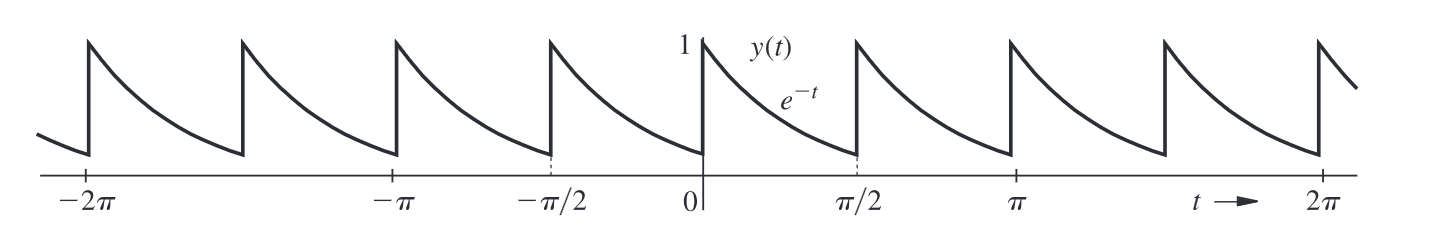
\includegraphics{assets/f1.png}

\[
f_{saw}(x) = 
  \sum_{k = -\infty}^{\infty} 
    1 * 
      (u(t - (k*10\pi - \pi)) - 
      u(t - (k*10\pi + \pi)))
\]

\hypertarget{sinal-2}{%
\subsection{Sinal 2}\label{sinal-2}}

\textbf{Figura P6.1-1 (d)}

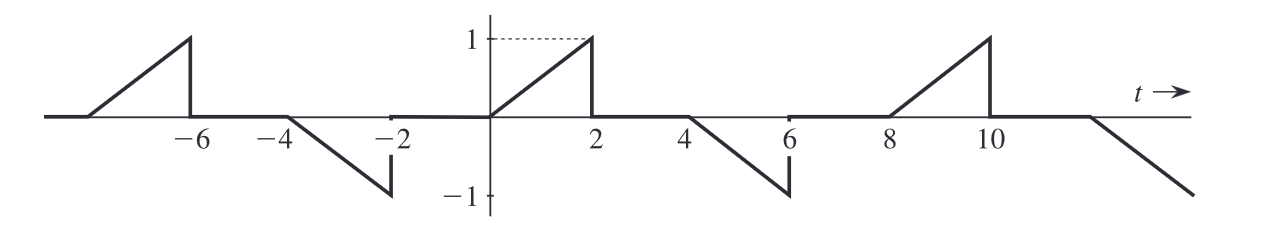
\includegraphics{assets/f2.png}

\[
f_{saw}(x) = \\
  \begin{cases} \\
    \frac{x}{2} & \quad \text{if }  0 <= x <= \frac{\pi}{4} \\
    \frac{-x}{2} & \quad \text{ if }  \frac{3\pi}{4} <= x <= \frac{4\pi}{4} \\
    \text{0, } & \quad \text{ otherwise} \\
  \end{cases}
\]

\textbf{Representação a função usando pulsos unitarios:}

\[
f_{saw}(x) = 
  \sum_{k = -\infty}^{\infty} 
    \frac{x - \pi k}{2} * 
      (u(t - \pi k) - 
      u(t - (\pi k + \frac{\pi}{4}))) +
    \frac{x - \pi k}{2} * 
      (u(t - (\pi k + \frac{3\pi}{4})) - 
      u(t - (\pi k + \frac{4\pi}{4})))       
\]

    \hypertarget{bibliotecas-utilizadas-no-cuxf3digo}{%
\section{Bibliotecas utilizadas no
código}\label{bibliotecas-utilizadas-no-cuxf3digo}}

    \begin{tcolorbox}[breakable, size=fbox, boxrule=1pt, pad at break*=1mm,colback=cellbackground, colframe=cellborder]
\prompt{In}{incolor}{1}{\boxspacing}
\begin{Verbatim}[commandchars=\\\{\}]
\PY{c+c1}{\PYZsh{} Packages install}
\PY{o}{\PYZpc{}}\PY{k}{pip} install \PYZhy{}q numpy control matplotlib scipy sympy
\end{Verbatim}
\end{tcolorbox}

    \begin{Verbatim}[commandchars=\\\{\}]
Note: you may need to restart the kernel to use updated packages.
    \end{Verbatim}

    \begin{tcolorbox}[breakable, size=fbox, boxrule=1pt, pad at break*=1mm,colback=cellbackground, colframe=cellborder]
\prompt{In}{incolor}{2}{\boxspacing}
\begin{Verbatim}[commandchars=\\\{\}]
\PY{c+c1}{\PYZsh{} Análise numérica}
\PY{k+kn}{import} \PY{n+nn}{numpy} \PY{k}{as} \PY{n+nn}{np}
\PY{c+c1}{\PYZsh{} Análise analitica}
\PY{k+kn}{import} \PY{n+nn}{sympy} \PY{k}{as} \PY{n+nn}{sym}
\PY{c+c1}{\PYZsh{} Plots}
\PY{k+kn}{import} \PY{n+nn}{matplotlib}\PY{n+nn}{.}\PY{n+nn}{pyplot} \PY{k}{as} \PY{n+nn}{plt}
\PY{k+kn}{from} \PY{n+nn}{matplotlib}\PY{n+nn}{.}\PY{n+nn}{ticker} \PY{k+kn}{import} \PY{n}{FormatStrFormatter}
\PY{c+c1}{\PYZsh{} Tipagem}
\PY{k+kn}{from} \PY{n+nn}{typing} \PY{k+kn}{import} \PY{n}{List}\PY{p}{,} \PY{n}{Tuple}
\PY{c+c1}{\PYZsh{} Desabilitar warnings (somente para exportação)}
\PY{k+kn}{import} \PY{n+nn}{warnings}
\PY{n}{warnings}\PY{o}{.}\PY{n}{filterwarnings}\PY{p}{(}\PY{l+s+s1}{\PYZsq{}}\PY{l+s+s1}{ignore}\PY{l+s+s1}{\PYZsq{}}\PY{p}{)}
\end{Verbatim}
\end{tcolorbox}

    \hypertarget{verificauxe7uxe3o-do-sinal-1}{%
\section{Verificação do Sinal 1}\label{verificauxe7uxe3o-do-sinal-1}}

\textbf{Figura P6.1-1 (b)}

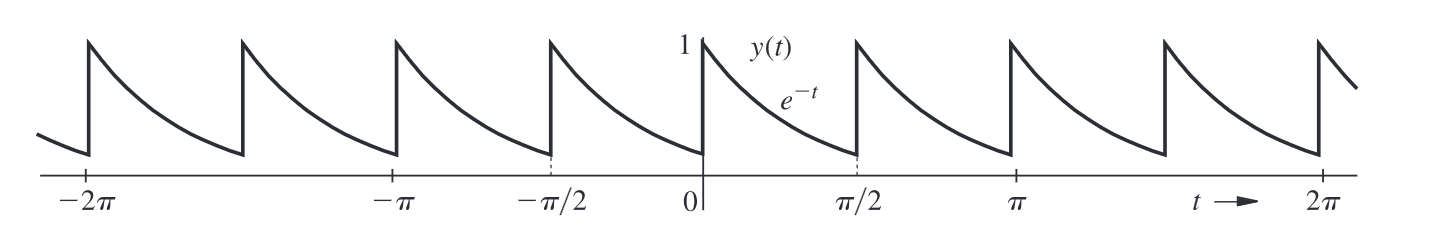
\includegraphics{assets/f1.png}

Para representar a função com um período de \(10\pi\), utiliza-se uma
função base constante igual a \(1\), multiplicada por duas funções
degrau unitário que definem o período. Dessa forma, o sinal é descrito
como sendo igual a \(1\) dentro do intervalo definido pelos dois degraus
unitários e igual a \(0\) fora desse intervalo.

\[
f_{saw}(x) = 
  \sum_{k = -\infty}^{\infty} 
    1 * 
      (u(t - (k*10\pi - \pi)) - 
      u(t - (k*10\pi + \pi)))
\]

    \hypertarget{descriuxe7uxe3o-em-cuxf3digo-da-funuxe7uxe3o}{%
\subsection{Descrição em código da
função}\label{descriuxe7uxe3o-em-cuxf3digo-da-funuxe7uxe3o}}

    \begin{tcolorbox}[breakable, size=fbox, boxrule=1pt, pad at break*=1mm,colback=cellbackground, colframe=cellborder]
\prompt{In}{incolor}{3}{\boxspacing}
\begin{Verbatim}[commandchars=\\\{\}]
\PY{k}{def} \PY{n+nf}{f\PYZus{}aux}\PY{p}{(}\PY{n}{x}\PY{p}{,} \PY{n}{k}\PY{p}{)}\PY{p}{:}
    \PY{k}{return} \PY{l+m+mi}{1} \PY{o}{*} \PY{p}{(}\PY{n}{np}\PY{o}{.}\PY{n}{heaviside}\PY{p}{(}\PY{n}{x} \PY{o}{\PYZhy{}} \PY{p}{(}\PY{n}{k} \PY{o}{*} \PY{p}{(}\PY{l+m+mi}{10} \PY{o}{*} \PY{n}{np}\PY{o}{.}\PY{n}{pi}\PY{p}{)} \PY{o}{\PYZhy{}} \PY{p}{(}\PY{n}{np}\PY{o}{.}\PY{n}{pi}\PY{p}{)}\PY{p}{)}\PY{p}{,} \PY{l+m+mi}{1}\PY{p}{)}\PY{p}{)} \PY{o}{\PYZhy{}} \PY{n}{np}\PY{o}{.}\PY{n}{heaviside}\PY{p}{(}\PY{n}{x} \PY{o}{\PYZhy{}} \PY{p}{(}\PY{n}{k} \PY{o}{*} \PY{p}{(}\PY{l+m+mi}{10} \PY{o}{*} \PY{n}{np}\PY{o}{.}\PY{n}{pi}\PY{p}{)} \PY{o}{+} \PY{p}{(}\PY{n}{np}\PY{o}{.}\PY{n}{pi}\PY{p}{)}\PY{p}{)}\PY{p}{,} \PY{l+m+mi}{1}\PY{p}{)}

\PY{k}{def} \PY{n+nf}{f}\PY{p}{(}\PY{n}{x}\PY{p}{)}\PY{p}{:}
    \PY{k}{return} \PY{p}{[}\PY{n}{np}\PY{o}{.}\PY{n}{sum}\PY{p}{(}\PY{p}{[} \PY{n}{f\PYZus{}aux}\PY{p}{(}\PY{n}{d}\PY{p}{,} \PY{n}{k}\PY{p}{)} \PY{k}{for} \PY{n}{k} \PY{o+ow}{in} \PY{n+nb}{range}\PY{p}{(}\PY{n+nb}{int}\PY{p}{(}\PY{n}{x}\PY{o}{.}\PY{n}{min}\PY{p}{(}\PY{p}{)} \PY{o}{/} \PY{p}{(}\PY{l+m+mi}{10} \PY{o}{*} \PY{n}{np}\PY{o}{.}\PY{n}{pi}\PY{p}{)}\PY{p}{)} \PY{o}{\PYZhy{}} \PY{l+m+mi}{2}\PY{p}{,} \PY{n+nb}{int}\PY{p}{(}\PY{n}{x}\PY{o}{.}\PY{n}{max}\PY{p}{(}\PY{p}{)} \PY{o}{/} \PY{p}{(}\PY{l+m+mi}{10} \PY{o}{*} \PY{n}{np}\PY{o}{.}\PY{n}{pi}\PY{p}{)}\PY{p}{)} \PY{o}{+} \PY{l+m+mi}{2}\PY{p}{)} \PY{p}{]}\PY{p}{)} \PY{k}{for} \PY{n}{d} \PY{o+ow}{in} \PY{n}{x} \PY{p}{]}
\end{Verbatim}
\end{tcolorbox}

    \hypertarget{gruxe1fico-do-sinal-1}{%
\subsection{Gráfico do Sinal 1}\label{gruxe1fico-do-sinal-1}}

    \begin{tcolorbox}[breakable, size=fbox, boxrule=1pt, pad at break*=1mm,colback=cellbackground, colframe=cellborder]
\prompt{In}{incolor}{4}{\boxspacing}
\begin{Verbatim}[commandchars=\\\{\}]
\PY{n}{x} \PY{o}{=} \PY{n}{np}\PY{o}{.}\PY{n}{linspace}\PY{p}{(}\PY{l+m+mi}{2} \PY{o}{*} \PY{o}{\PYZhy{}}\PY{l+m+mi}{10} \PY{o}{*} \PY{n}{np}\PY{o}{.}\PY{n}{pi}\PY{p}{,} \PY{l+m+mi}{2} \PY{o}{*} \PY{l+m+mi}{10} \PY{o}{*} \PY{n}{np}\PY{o}{.}\PY{n}{pi}\PY{p}{,} \PY{l+m+mi}{10000}\PY{p}{)}
\PY{n}{y} \PY{o}{=} \PY{n}{f}\PY{p}{(}\PY{n}{x}\PY{p}{)}

\PY{n}{fig} \PY{o}{=} \PY{n}{plt}\PY{o}{.}\PY{n}{figure}\PY{p}{(}\PY{n}{figsize} \PY{o}{=} \PY{p}{(}\PY{l+m+mi}{25}\PY{p}{,} \PY{l+m+mi}{8}\PY{p}{)}\PY{p}{)}
\PY{n}{ax} \PY{o}{=} \PY{n}{fig}\PY{o}{.}\PY{n}{add\PYZus{}subplot}\PY{p}{(}\PY{p}{)}
\PY{n}{ax}\PY{o}{.}\PY{n}{grid}\PY{p}{(}\PY{p}{)}
\PY{n}{ax}\PY{o}{.}\PY{n}{plot}\PY{p}{(}\PY{n}{x}\PY{p}{,} \PY{n}{y}\PY{p}{)}


\PY{c+c1}{\PYZsh{} Configurando o grafico}

\PY{n}{ax}\PY{o}{.}\PY{n}{set\PYZus{}title}\PY{p}{(}\PY{l+s+sa}{f}\PY{l+s+s1}{\PYZsq{}}\PY{l+s+s1}{f(x)}\PY{l+s+s1}{\PYZsq{}}\PY{p}{)}
\PY{n}{ax}\PY{o}{.}\PY{n}{set\PYZus{}xticks}\PY{p}{(}\PY{n}{np}\PY{o}{.}\PY{n}{arange}\PY{p}{(}\PY{n}{x}\PY{o}{.}\PY{n}{min}\PY{p}{(}\PY{p}{)}\PY{p}{,} \PY{n}{x}\PY{o}{.}\PY{n}{max}\PY{p}{(}\PY{p}{)}\PY{p}{,} \PY{n}{np}\PY{o}{.}\PY{n}{pi}\PY{p}{)}\PY{p}{)}
\PY{n}{ax}\PY{o}{.}\PY{n}{xaxis}\PY{o}{.}\PY{n}{set\PYZus{}major\PYZus{}formatter}\PY{p}{(}\PY{n}{FormatStrFormatter}\PY{p}{(}\PY{l+s+s1}{\PYZsq{}}\PY{l+s+si}{\PYZpc{}.1f}\PY{l+s+s1}{\PYZsq{}}\PY{p}{)}\PY{p}{)}
\PY{n}{ax}\PY{o}{.}\PY{n}{grid}\PY{p}{(}\PY{n}{visible}\PY{o}{=}\PY{k+kc}{True}\PY{p}{)}
\end{Verbatim}
\end{tcolorbox}

    \begin{center}
    \adjustimage{max size={0.9\linewidth}{0.9\paperheight}}{fourier_files/fourier_9_0.png}
    \end{center}
    { \hspace*{\fill} \\}
    
    \hypertarget{calculando-os-coeficientes-da-suxe9rie-de-fourier---item-1}{%
\subsection{Calculando os coeficientes da série de Fourier - Item
1}\label{calculando-os-coeficientes-da-suxe9rie-de-fourier---item-1}}

Os coeficientes da série de Fourier podem ser calculados utilizando a
seguinte fórmula:

\[ck(k) = \frac{1}{T_0} \int_{T_0} f(x)e^{-j w_0 t}dt\]

Ao substituir a função na integral, temos:

\[ck(k) = \frac{1}{T_0} \int_{T_0} 1 e^{-j w_0 t}dt\]

Considerando que a função é composta por partes, podemos expressá-la
como a soma de integrais:

\[
ck(k) = \frac{1}{T_0} \int_{0}^{\pi} 1 e^{-j w_0 t}dt +
\frac{1}{T_0} \int_{\pi}^{9\pi} 0 * e^{-j w_0 t}dt +
\frac{1}{T_0} \int_{9\pi}^{10\pi} 1 e^{-j w_0 t}dt
\]

Resolvendo a integral:

\[\begin{cases} \frac{i \left(e^{\frac{19 i \pi k}{5}} - e^{\frac{11 i \pi k}{5}} - e^{4 i \pi k} + e^{2 i \pi k}\right) e^{- 4 i \pi k}}{2 \pi k} & \text{for}\: \left(k > -\infty \vee k > 0\right) \wedge \left(k > -\infty \vee k < \infty\right) \wedge \left(k > 0 \vee k < 0\right) \wedge \left(k < 0 \vee k < \infty\right) \\\frac{1}{5} & \text{otherwise} \end{cases}\]

    \begin{tcolorbox}[breakable, size=fbox, boxrule=1pt, pad at break*=1mm,colback=cellbackground, colframe=cellborder]
\prompt{In}{incolor}{5}{\boxspacing}
\begin{Verbatim}[commandchars=\\\{\}]
\PY{c+c1}{\PYZsh{} Periodo}
\PY{n}{t\PYZus{}0} \PY{o}{=} \PY{l+m+mi}{10} \PY{o}{*} \PY{n}{sym}\PY{o}{.}\PY{n}{pi}
\PY{c+c1}{\PYZsh{} Frequencia}
\PY{n}{f\PYZus{}0} \PY{o}{=} \PY{l+m+mi}{1} \PY{o}{/} \PY{n}{t\PYZus{}0}
\PY{c+c1}{\PYZsh{} Frequencia angular}
\PY{n}{w\PYZus{}0} \PY{o}{=} \PY{l+m+mi}{2} \PY{o}{*} \PY{n}{sym}\PY{o}{.}\PY{n}{pi} \PY{o}{*} \PY{n}{f\PYZus{}0}

\PY{c+c1}{\PYZsh{} Definindo a variavel independente}
\PY{n}{t} \PY{o}{=} \PY{n}{sym}\PY{o}{.}\PY{n}{Symbol}\PY{p}{(}\PY{l+s+s1}{\PYZsq{}}\PY{l+s+s1}{t}\PY{l+s+s1}{\PYZsq{}}\PY{p}{)}
\PY{c+c1}{\PYZsh{} Definindo o periodo}
\PY{n}{k} \PY{o}{=} \PY{n}{sym}\PY{o}{.}\PY{n}{Symbol}\PY{p}{(}\PY{l+s+s1}{\PYZsq{}}\PY{l+s+s1}{k}\PY{l+s+s1}{\PYZsq{}}\PY{p}{)}

\PY{c+c1}{\PYZsh{} Calculando a equação que define os coeficientes da serie de fourier para a função}
\PY{n}{ck} \PY{o}{=} \PY{n}{f\PYZus{}0} \PY{o}{*} \PY{n}{sym}\PY{o}{.}\PY{n}{integrate}\PY{p}{(}\PY{l+m+mi}{1} \PY{o}{*} \PY{n}{sym}\PY{o}{.}\PY{n}{exp}\PY{p}{(}\PY{o}{\PYZhy{}}\PY{n}{sym}\PY{o}{.}\PY{n}{I} \PY{o}{*} \PY{n}{k} \PY{o}{*} \PY{n}{w\PYZus{}0} \PY{o}{*} \PY{n}{t}\PY{p}{)}\PY{p}{,} \PY{p}{(}\PY{n}{t}\PY{p}{,} \PY{l+m+mi}{0}\PY{p}{,} \PY{n}{sym}\PY{o}{.}\PY{n}{pi}\PY{p}{)}\PY{p}{)} \PY{o}{+} \PYZbs{}
    \PY{n}{f\PYZus{}0} \PY{o}{*} \PY{n}{sym}\PY{o}{.}\PY{n}{integrate}\PY{p}{(}\PY{l+m+mi}{0} \PY{o}{*} \PY{n}{sym}\PY{o}{.}\PY{n}{exp}\PY{p}{(}\PY{o}{\PYZhy{}}\PY{n}{sym}\PY{o}{.}\PY{n}{I} \PY{o}{*} \PY{n}{k} \PY{o}{*} \PY{n}{w\PYZus{}0} \PY{o}{*} \PY{n}{t}\PY{p}{)}\PY{p}{,} \PY{p}{(}\PY{n}{t}\PY{p}{,} \PY{n}{sym}\PY{o}{.}\PY{n}{pi} \PY{p}{,} \PY{l+m+mi}{9} \PY{o}{*} \PY{n}{sym}\PY{o}{.}\PY{n}{pi}\PY{p}{)}\PY{p}{)} \PY{o}{+} \PYZbs{}
    \PY{n}{f\PYZus{}0} \PY{o}{*} \PY{n}{sym}\PY{o}{.}\PY{n}{integrate}\PY{p}{(}\PY{l+m+mi}{1} \PY{o}{*} \PY{n}{sym}\PY{o}{.}\PY{n}{exp}\PY{p}{(}\PY{o}{\PYZhy{}}\PY{n}{sym}\PY{o}{.}\PY{n}{I} \PY{o}{*} \PY{n}{k} \PY{o}{*} \PY{n}{w\PYZus{}0} \PY{o}{*} \PY{n}{t}\PY{p}{)}\PY{p}{,} \PY{p}{(}\PY{n}{t}\PY{p}{,} \PY{l+m+mi}{9} \PY{o}{*} \PY{n}{sym}\PY{o}{.}\PY{n}{pi} \PY{p}{,} \PY{l+m+mi}{10} \PY{o}{*} \PY{n}{sym}\PY{o}{.}\PY{n}{pi}\PY{p}{)}\PY{p}{)}

\PY{n+nb}{print}\PY{p}{(}\PY{l+s+s2}{\PYZdq{}}\PY{l+s+s2}{Coeficientes da serie de fourier:}\PY{l+s+s2}{\PYZdq{}}\PY{p}{)}
\PY{n}{display}\PY{p}{(}\PY{n}{sym}\PY{o}{.}\PY{n}{simplify}\PY{p}{(}\PY{n}{ck}\PY{p}{)}\PY{p}{)}
\end{Verbatim}
\end{tcolorbox}

    \begin{Verbatim}[commandchars=\\\{\}]
Coeficientes da serie de fourier:
    \end{Verbatim}

    $\displaystyle \begin{cases} \frac{i \left(e^{\frac{19 i \pi k}{5}} - e^{\frac{11 i \pi k}{5}} - e^{4 i \pi k} + e^{2 i \pi k}\right) e^{- 4 i \pi k}}{2 \pi k} & \text{for}\: \left(k > -\infty \vee k > 0\right) \wedge \left(k > -\infty \vee k < \infty\right) \wedge \left(k > 0 \vee k < 0\right) \wedge \left(k < 0 \vee k < \infty\right) \\\frac{1}{5} & \text{otherwise} \end{cases}$

    
    \hypertarget{recriauxe7uxe3o-do-sinal-a-partir-da-suxe9rie-de-fourier---item-2}{%
\subsection{Recriação do sinal a partir da série de Fourier - Item
2}\label{recriauxe7uxe3o-do-sinal-a-partir-da-suxe9rie-de-fourier---item-2}}

    \hypertarget{cuxe1lculo-de-recriauxe7uxe3o}{%
\subsubsection{Cálculo de
recriação}\label{cuxe1lculo-de-recriauxe7uxe3o}}

Usando a função, são criadas `ks\_len' harmônicas para cada amostra de
tempo `t', a fim de recriar a função.

\[ 
f_{new}(t) =
\sum_{k = -\infty}^{\infty}
c_k(k) * e^{k j w_0 t}
\]

Para alcançar esse objetivo, é criada uma função que recebe dois
vetores: um vetor de harmônicas e um vetor de amostras de tempo. Em
seguida, realiza-se a soma descrita acima para cada amostra `t' presente
no vetor de tempo.

    \begin{tcolorbox}[breakable, size=fbox, boxrule=1pt, pad at break*=1mm,colback=cellbackground, colframe=cellborder]
\prompt{In}{incolor}{6}{\boxspacing}
\begin{Verbatim}[commandchars=\\\{\}]
\PY{k}{def} \PY{n+nf}{f\PYZus{}t\PYZus{}new}\PY{p}{(}\PY{n}{ks}\PY{p}{,} \PY{n}{t}\PY{p}{)}\PY{p}{:}
    \PY{c+c1}{\PYZsh{} Converte a equação que define os coeficientes da serie de fourier para uma função ck(k)}
    \PY{n}{ck\PYZus{}k} \PY{o}{=} \PY{n}{sym}\PY{o}{.}\PY{n}{lambdify}\PY{p}{(}\PY{n}{k}\PY{p}{,} \PY{n}{ck}\PY{p}{)}
    \PY{c+c1}{\PYZsh{} Criando matriz de t com tamanho k para calcular a somatoria}
    \PY{n}{t\PYZus{}m} \PY{o}{=} \PY{n}{np}\PY{o}{.}\PY{n}{tile}\PY{p}{(}\PY{n}{t}\PY{p}{,} \PY{p}{(}\PY{n+nb}{len}\PY{p}{(}\PY{n}{ks}\PY{p}{)}\PY{p}{,} \PY{l+m+mi}{1}\PY{p}{)}\PY{p}{)}

    \PY{c+c1}{\PYZsh{} Recriando a função de t a partir da serie de fourier}
    \PY{k}{return} \PY{n}{np}\PY{o}{.}\PY{n}{sum}\PY{p}{(}\PY{n}{np}\PY{o}{.}\PY{n}{transpose}\PY{p}{(}\PY{n}{ck\PYZus{}k}\PY{p}{(}\PY{n}{ks}\PY{p}{)}\PY{p}{)}\PY{p}{[}\PY{p}{:}\PY{p}{,} \PY{n}{np}\PY{o}{.}\PY{n}{newaxis}\PY{p}{]} \PY{o}{*} \PY{n}{np}\PY{o}{.}\PY{n}{exp}\PY{p}{(}\PY{l+m+mi}{1}\PY{n}{j} \PY{o}{*} \PY{n}{np}\PY{o}{.}\PY{n}{transpose}\PY{p}{(}\PY{n}{ks}\PY{p}{)}\PY{p}{[}\PY{p}{:}\PY{p}{,} \PY{n}{np}\PY{o}{.}\PY{n}{newaxis}\PY{p}{]} \PY{o}{*} \PY{n+nb}{float}\PY{p}{(}\PY{n}{w\PYZus{}0}\PY{p}{)} \PY{o}{*} \PY{n}{t\PYZus{}m}\PY{p}{)}\PY{p}{,} \PY{n}{axis}\PY{o}{=}\PY{l+m+mi}{0}\PY{p}{)}
\end{Verbatim}
\end{tcolorbox}

    \hypertarget{gruxe1fico-das-funuxe7uxf5es-original-e-reconstruuxedda}{%
\subsubsection{Gráfico das funções original e
reconstruída}\label{gruxe1fico-das-funuxe7uxf5es-original-e-reconstruuxedda}}

O gráfico que descreve a função reconstruída e a função original para
diferentes números de harmônicas `k' é apresentado abaixo:

    \begin{tcolorbox}[breakable, size=fbox, boxrule=1pt, pad at break*=1mm,colback=cellbackground, colframe=cellborder]
\prompt{In}{incolor}{7}{\boxspacing}
\begin{Verbatim}[commandchars=\\\{\}]
\PY{c+c1}{\PYZsh{} Numero de periodos}
\PY{n}{t\PYZus{}len} \PY{o}{=} \PY{l+m+mi}{4}

\PY{c+c1}{\PYZsh{} Criando um vetor de t}
\PY{n}{t} \PY{o}{=} \PY{n}{np}\PY{o}{.}\PY{n}{linspace}\PY{p}{(}\PY{o}{\PYZhy{}}\PY{p}{(}\PY{n}{t\PYZus{}len} \PY{o}{/} \PY{l+m+mi}{2}\PY{p}{)} \PY{o}{*} \PY{n+nb}{float}\PY{p}{(}\PY{n}{t\PYZus{}0}\PY{p}{)}\PY{p}{,} \PY{p}{(}\PY{n}{t\PYZus{}len} \PY{o}{/} \PY{l+m+mi}{2}\PY{p}{)} \PY{o}{*} \PY{n+nb}{float}\PY{p}{(}\PY{n}{t\PYZus{}0}\PY{p}{)}\PY{p}{,} \PY{l+m+mi}{1000}\PY{p}{)}

\PY{c+c1}{\PYZsh{} Cria a figura e o plot e ativa o grid}
\PY{n}{fig}\PY{p}{,} \PY{n}{axs} \PY{o}{=} \PY{n}{plt}\PY{o}{.}\PY{n}{subplots}\PY{p}{(}\PY{l+m+mi}{5}\PY{p}{,} \PY{l+m+mi}{1}\PY{p}{,} \PY{n}{figsize} \PY{o}{=} \PY{p}{(}\PY{l+m+mi}{18}\PY{p}{,} \PY{l+m+mi}{15}\PY{p}{)}\PY{p}{)}
\PY{n}{fig}\PY{o}{.}\PY{n}{subplots\PYZus{}adjust}\PY{p}{(}\PY{n}{hspace}\PY{o}{=}\PY{l+m+mf}{0.5}\PY{p}{)}



\PY{k}{for} \PY{n}{i}\PY{p}{,} \PY{n}{ax} \PY{o+ow}{in} \PY{n+nb}{enumerate}\PY{p}{(}\PY{n}{axs}\PY{p}{)}\PY{p}{:}

    \PY{c+c1}{\PYZsh{} Calculando para o numero de harmonicos}
    \PY{c+c1}{\PYZsh{} Numero de harmonicas}
    \PY{n}{ks\PYZus{}len} \PY{o}{=} \PY{n+nb}{int}\PY{p}{(}\PY{l+m+mi}{100} \PY{o}{/} \PY{p}{(}\PY{l+m+mi}{2} \PY{o}{*}\PY{o}{*} \PY{n}{i}\PY{p}{)}\PY{p}{)}

    \PY{c+c1}{\PYZsh{} Criando um vetor de harmonicas}
    \PY{n}{ks} \PY{o}{=} \PY{n}{np}\PY{o}{.}\PY{n}{arange}\PY{p}{(}\PY{o}{\PYZhy{}}\PY{n+nb}{int}\PY{p}{(}\PY{n}{ks\PYZus{}len} \PY{o}{/} \PY{l+m+mi}{2}\PY{p}{)}\PY{p}{,} \PY{n+nb}{int}\PY{p}{(}\PY{n}{ks\PYZus{}len} \PY{o}{/} \PY{l+m+mi}{2}\PY{p}{)}\PY{p}{,} \PY{l+m+mi}{1}\PY{p}{)}

    \PY{c+c1}{\PYZsh{} Configurando o grafico}
    \PY{n}{ax}\PY{o}{.}\PY{n}{set\PYZus{}title}\PY{p}{(}\PY{l+s+sa}{f}\PY{l+s+s1}{\PYZsq{}}\PY{l+s+s1}{f(x) n\PYZus{}harmonicos: }\PY{l+s+si}{\PYZob{}}\PY{n}{ks\PYZus{}len}\PY{l+s+si}{\PYZcb{}}\PY{l+s+s1}{\PYZsq{}}\PY{p}{)}
    \PY{n}{ax}\PY{o}{.}\PY{n}{set\PYZus{}xticks}\PY{p}{(}\PY{n}{np}\PY{o}{.}\PY{n}{arange}\PY{p}{(}\PY{o}{\PYZhy{}}\PY{p}{(}\PY{n}{t\PYZus{}len} \PY{o}{*} \PY{n+nb}{float}\PY{p}{(}\PY{n}{t\PYZus{}0}\PY{p}{)}\PY{p}{)}\PY{p}{,} \PY{p}{(}\PY{n}{t\PYZus{}len} \PY{o}{*} \PY{n+nb}{float}\PY{p}{(}\PY{n}{t\PYZus{}0}\PY{p}{)}\PY{p}{)}\PY{p}{,} \PY{n+nb}{float}\PY{p}{(}\PY{n}{t\PYZus{}0}\PY{p}{)} \PY{o}{/} \PY{l+m+mi}{2}\PY{p}{)}\PY{p}{)}
    \PY{n}{ax}\PY{o}{.}\PY{n}{grid}\PY{p}{(}\PY{p}{)}

    \PY{c+c1}{\PYZsh{} Desenha o grafico da onda real}
    \PY{n}{ax}\PY{o}{.}\PY{n}{plot}\PY{p}{(}\PY{n}{t}\PY{p}{,} \PY{n}{f}\PY{p}{(}\PY{n}{t}\PY{p}{)}\PY{p}{,} \PY{n}{label}\PY{o}{=}\PY{l+s+s1}{\PYZsq{}}\PY{l+s+s1}{real}\PY{l+s+s1}{\PYZsq{}}\PY{p}{)}   

    \PY{c+c1}{\PYZsh{} Cria o grafico da onda estimada pela serie}
    \PY{n}{ax}\PY{o}{.}\PY{n}{plot}\PY{p}{(}\PY{n}{t}\PY{p}{,} \PY{n}{f\PYZus{}t\PYZus{}new}\PY{p}{(}\PY{n}{ks}\PY{p}{,} \PY{n}{t}\PY{p}{)}\PY{p}{,} \PY{n}{label}\PY{o}{=}\PY{l+s+s1}{\PYZsq{}}\PY{l+s+s1}{serie}\PY{l+s+s1}{\PYZsq{}}\PY{p}{)}

    \PY{n}{ax}\PY{o}{.}\PY{n}{legend}\PY{p}{(}\PY{p}{)}

\PY{c+c1}{\PYZsh{} Show the plot}
\PY{n}{plt}\PY{o}{.}\PY{n}{show}\PY{p}{(}\PY{p}{)}
\end{Verbatim}
\end{tcolorbox}

    \begin{center}
    \adjustimage{max size={0.9\linewidth}{0.9\paperheight}}{fourier_files/fourier_16_0.png}
    \end{center}
    { \hspace*{\fill} \\}
    
    \hypertarget{desenho-do-grafico-para-um-numero-de-harmonicas-especifico-item-3}{%
\subsection{Desenho do grafico para um numero de harmonicas especifico
(item
3)}\label{desenho-do-grafico-para-um-numero-de-harmonicas-especifico-item-3}}

Para realizar o desenho do gráfico para um número específico de
harmônicas, esta célula solicita ao usuário que informe a quantidade
desejada. Em seguida, o código plota o gráfico correspondente a essa
quantidade de harmônicas.

Importante: É necessário executar as células anteriores para que esta
funcionalidade esteja disponível.

    \begin{tcolorbox}[breakable, size=fbox, boxrule=1pt, pad at break*=1mm,colback=cellbackground, colframe=cellborder]
\prompt{In}{incolor}{8}{\boxspacing}
\begin{Verbatim}[commandchars=\\\{\}]
\PY{c+c1}{\PYZsh{} Numero de periodos}
\PY{n}{t\PYZus{}len} \PY{o}{=} \PY{l+m+mi}{3}

\PY{c+c1}{\PYZsh{} Criando um vetor de t}
\PY{n}{t} \PY{o}{=} \PY{n}{np}\PY{o}{.}\PY{n}{linspace}\PY{p}{(}\PY{o}{\PYZhy{}}\PY{p}{(}\PY{n}{t\PYZus{}len} \PY{o}{/} \PY{l+m+mi}{2}\PY{p}{)} \PY{o}{*} \PY{n+nb}{float}\PY{p}{(}\PY{n}{t\PYZus{}0}\PY{p}{)}\PY{p}{,} \PY{p}{(}\PY{n}{t\PYZus{}len} \PY{o}{/} \PY{l+m+mi}{2}\PY{p}{)} \PY{o}{*} \PY{n+nb}{float}\PY{p}{(}\PY{n}{t\PYZus{}0}\PY{p}{)}\PY{p}{,} \PY{l+m+mi}{10000}\PY{p}{)}

\PY{n}{fig} \PY{o}{=} \PY{n}{plt}\PY{o}{.}\PY{n}{figure}\PY{p}{(}\PY{n}{figsize} \PY{o}{=} \PY{p}{(}\PY{l+m+mi}{18}\PY{p}{,} \PY{l+m+mi}{8}\PY{p}{)}\PY{p}{)}
\PY{n}{ax} \PY{o}{=} \PY{n}{fig}\PY{o}{.}\PY{n}{subplots}\PY{p}{(}\PY{p}{)}
\PY{c+c1}{\PYZsh{} Numero de harmonicas}
\PY{n}{ks\PYZus{}len} \PY{o}{=} \PY{n+nb}{int}\PY{p}{(}\PY{n+nb}{input}\PY{p}{(}\PY{l+s+s1}{\PYZsq{}}\PY{l+s+s1}{Numero de harmonicas}\PY{l+s+s1}{\PYZsq{}}\PY{p}{)}\PY{p}{)}

\PY{c+c1}{\PYZsh{} Criando um vetor de harmonicas}
\PY{n}{ks} \PY{o}{=} \PY{n}{np}\PY{o}{.}\PY{n}{arange}\PY{p}{(}\PY{o}{\PYZhy{}}\PY{n+nb}{int}\PY{p}{(}\PY{n}{ks\PYZus{}len} \PY{o}{/} \PY{l+m+mi}{2}\PY{p}{)}\PY{p}{,} \PY{n+nb}{int}\PY{p}{(}\PY{n}{ks\PYZus{}len} \PY{o}{/} \PY{l+m+mi}{2}\PY{p}{)}\PY{p}{,} \PY{l+m+mi}{1}\PY{p}{)}

\PY{n}{ax}\PY{o}{.}\PY{n}{set\PYZus{}title}\PY{p}{(}\PY{l+s+sa}{f}\PY{l+s+s1}{\PYZsq{}}\PY{l+s+s1}{f(x) n\PYZus{}harmonicos: }\PY{l+s+si}{\PYZob{}}\PY{n}{ks\PYZus{}len}\PY{l+s+si}{\PYZcb{}}\PY{l+s+s1}{\PYZsq{}}\PY{p}{)}
\PY{n}{ax}\PY{o}{.}\PY{n}{set\PYZus{}xticks}\PY{p}{(}\PY{n}{np}\PY{o}{.}\PY{n}{arange}\PY{p}{(}\PY{o}{\PYZhy{}}\PY{p}{(}\PY{n}{t\PYZus{}len} \PY{o}{*} \PY{n+nb}{float}\PY{p}{(}\PY{n}{t\PYZus{}0}\PY{p}{)}\PY{p}{)}\PY{p}{,} \PY{p}{(}\PY{n}{t\PYZus{}len} \PY{o}{*} \PY{n+nb}{float}\PY{p}{(}\PY{n}{t\PYZus{}0}\PY{p}{)}\PY{p}{)}\PY{p}{,} \PY{n+nb}{float}\PY{p}{(}\PY{n}{t\PYZus{}0}\PY{p}{)} \PY{o}{/} \PY{l+m+mi}{10}\PY{p}{)}\PY{p}{)}

\PY{c+c1}{\PYZsh{} Cria o grafico da onda estimada pela serie}
\PY{n}{ax}\PY{o}{.}\PY{n}{plot}\PY{p}{(}\PY{n}{t}\PY{p}{,} \PY{n}{f\PYZus{}t\PYZus{}new}\PY{p}{(}\PY{n}{ks}\PY{p}{,} \PY{n}{t}\PY{p}{)}\PY{p}{,} \PY{n}{label}\PY{o}{=}\PY{l+s+s1}{\PYZsq{}}\PY{l+s+s1}{serie}\PY{l+s+s1}{\PYZsq{}}\PY{p}{)}
\PY{n}{ax}\PY{o}{.}\PY{n}{grid}\PY{p}{(}\PY{p}{)}
\end{Verbatim}
\end{tcolorbox}

    \begin{center}
    \adjustimage{max size={0.9\linewidth}{0.9\paperheight}}{fourier_files/fourier_18_0.png}
    \end{center}
    { \hspace*{\fill} \\}
    
    \hypertarget{gruxe1fico-da-magnitude-e-fase-dos-coeficientes}{%
\subsection{Gráfico da magnitude e fase dos
coeficientes}\label{gruxe1fico-da-magnitude-e-fase-dos-coeficientes}}

Neste gráfico, são representados a magnitude e a fase dos coeficientes
da série utilizando a função ck(k). No eixo X, estão os valores de `k'
(sendo `k' um número inteiro), enquanto no eixo Y são apresentados
\textbar Ck(k)\textbar{} e o ângulo de Ck(k) para os gráficos 1 e 2,
respectivamente.

    \begin{tcolorbox}[breakable, size=fbox, boxrule=1pt, pad at break*=1mm,colback=cellbackground, colframe=cellborder]
\prompt{In}{incolor}{9}{\boxspacing}
\begin{Verbatim}[commandchars=\\\{\}]
\PY{c+c1}{\PYZsh{} Converte a equação que define os coeficientes da serie de fourier para uma função ck(k)}
\PY{n}{ck\PYZus{}k} \PY{o}{=} \PY{n}{sym}\PY{o}{.}\PY{n}{lambdify}\PY{p}{(}\PY{n}{k}\PY{p}{,} \PY{n}{ck}\PY{p}{)}

\PY{c+c1}{\PYZsh{} Numero de harmonicas}
\PY{n}{ks\PYZus{}len} \PY{o}{=} \PY{l+m+mi}{50}

\PY{c+c1}{\PYZsh{} Criando um vetor de harmonicas}
\PY{n}{ks} \PY{o}{=} \PY{n}{np}\PY{o}{.}\PY{n}{arange}\PY{p}{(}\PY{o}{\PYZhy{}}\PY{n}{ks\PYZus{}len} \PY{o}{/} \PY{l+m+mi}{2}\PY{p}{,} \PY{n}{ks\PYZus{}len} \PY{o}{/} \PY{l+m+mi}{2}\PY{p}{,} \PY{l+m+mi}{1}\PY{p}{)}

\PY{n}{fig} \PY{o}{=} \PY{n}{plt}\PY{o}{.}\PY{n}{figure}\PY{p}{(}\PY{n}{figsize}\PY{o}{=}\PY{p}{(}\PY{l+m+mi}{18}\PY{p}{,} \PY{l+m+mi}{10}\PY{p}{)}\PY{p}{)}
\PY{p}{(}\PY{n}{ax}\PY{p}{,} \PY{n}{ax2}\PY{p}{)} \PY{o}{=} \PY{n}{fig}\PY{o}{.}\PY{n}{subplots}\PY{p}{(}\PY{l+m+mi}{2}\PY{p}{,} \PY{l+m+mi}{1}\PY{p}{)}
\PY{n}{ax}\PY{o}{.}\PY{n}{set\PYZus{}title}\PY{p}{(}\PY{l+s+s2}{\PYZdq{}}\PY{l+s+s2}{Magnitude e fase dos coeficientes da serie}\PY{l+s+s2}{\PYZdq{}}\PY{p}{)}

\PY{c+c1}{\PYZsh{} Grafico da magnitude dos coeficientes}
\PY{n}{ax}\PY{o}{.}\PY{n}{stem}\PY{p}{(}\PY{n}{ks}\PY{p}{,} \PY{n}{np}\PY{o}{.}\PY{n}{abs}\PY{p}{(}\PY{n}{ck\PYZus{}k}\PY{p}{(}\PY{n}{ks}\PY{p}{)}\PY{p}{)}\PY{p}{,} \PY{n}{label} \PY{o}{=} \PY{l+s+s1}{\PYZsq{}}\PY{l+s+s1}{|Ck|}\PY{l+s+s1}{\PYZsq{}}\PY{p}{)}
\PY{n}{ax}\PY{o}{.}\PY{n}{grid}\PY{p}{(}\PY{n}{alpha} \PY{o}{=} \PY{l+m+mf}{0.5}\PY{p}{)}
\PY{n}{ax}\PY{o}{.}\PY{n}{set\PYZus{}ylabel}\PY{p}{(}\PY{l+s+s2}{\PYZdq{}}\PY{l+s+s2}{|H(s)|}\PY{l+s+s2}{\PYZdq{}}\PY{p}{,} \PY{n}{weight} \PY{o}{=} \PY{l+s+s2}{\PYZdq{}}\PY{l+s+s2}{bold}\PY{l+s+s2}{\PYZdq{}}\PY{p}{)}
\PY{n}{ax}\PY{o}{.}\PY{n}{set\PYZus{}xticks}\PY{p}{(}\PY{n}{ks}\PY{p}{)}

\PY{c+c1}{\PYZsh{} Grafico da fase dos coeficientes}
\PY{c+c1}{\PYZsh{}ax2 = ax.twinx()}
\PY{n}{ax2}\PY{o}{.}\PY{n}{stem}\PY{p}{(}\PY{n}{ks}\PY{p}{,} \PY{n}{np}\PY{o}{.}\PY{n}{angle}\PY{p}{(}\PY{n}{ck\PYZus{}k}\PY{p}{(}\PY{n}{ks}\PY{p}{)}\PY{p}{)}\PY{p}{,} \PY{n}{label} \PY{o}{=} \PY{l+s+s1}{\PYZsq{}}\PY{l+s+s1}{Ck\PYZus{}fase}\PY{l+s+s1}{\PYZsq{}}\PY{p}{)}
\PY{n}{ax2}\PY{o}{.}\PY{n}{set\PYZus{}ylabel}\PY{p}{(}\PY{l+s+s2}{\PYZdq{}}\PY{l+s+s2}{fase(rad)}\PY{l+s+s2}{\PYZdq{}}\PY{p}{,} \PY{n}{weight} \PY{o}{=} \PY{l+s+s2}{\PYZdq{}}\PY{l+s+s2}{bold}\PY{l+s+s2}{\PYZdq{}}\PY{p}{)}
\PY{n}{ax2}\PY{o}{.}\PY{n}{set\PYZus{}xlabel}\PY{p}{(}\PY{l+s+s2}{\PYZdq{}}\PY{l+s+s2}{k}\PY{l+s+s2}{\PYZdq{}}\PY{p}{,} \PY{n}{weight} \PY{o}{=} \PY{l+s+s2}{\PYZdq{}}\PY{l+s+s2}{bold}\PY{l+s+s2}{\PYZdq{}}\PY{p}{)}
\PY{n}{ax2}\PY{o}{.}\PY{n}{set\PYZus{}xticks}\PY{p}{(}\PY{n}{ks}\PY{p}{)}
\PY{n}{ax2}\PY{o}{.}\PY{n}{grid}\PY{p}{(}\PY{n}{alpha} \PY{o}{=} \PY{l+m+mf}{0.5}\PY{p}{)}
\end{Verbatim}
\end{tcolorbox}

    \begin{center}
    \adjustimage{max size={0.9\linewidth}{0.9\paperheight}}{fourier_files/fourier_20_0.png}
    \end{center}
    { \hspace*{\fill} \\}
    
    \hypertarget{verificando-a-funuxe7uxe3o-2}{%
\section{Verificando a função 2}\label{verificando-a-funuxe7uxe3o-2}}

\textbf{Figura P6.1-1 (d)}

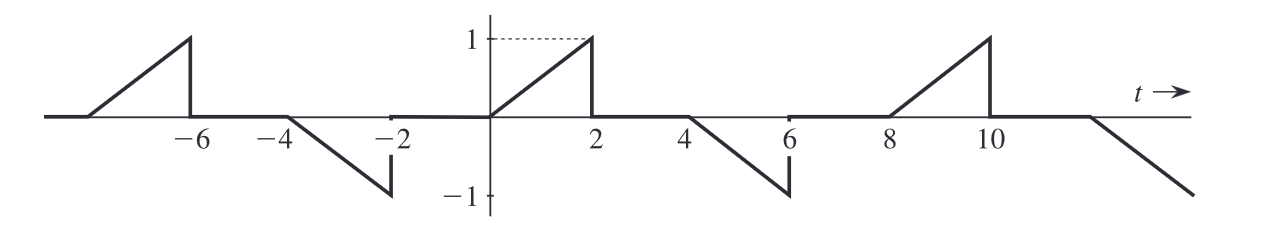
\includegraphics{assets/f2.png}

A função tem um periodo de \(\pi\) e em esse periodo é descrita por

\[
f_{saw}(x) = \\
  \begin{cases} \\
    \frac{x}{2} & \quad \text{if }  0 <= x <= \frac{\pi}{4} \\
    \frac{-x}{2} & \quad \text{ if }  \frac{3\pi}{4} <= x <= \frac{4\pi}{4} \\
    \text{0, } & \quad \text{ otherwise} \\
  \end{cases}
\]

\textbf{Representação a função usando pulsos unitarios:}

\[
f_{saw}(x) = 
  \sum_{k = -\infty}^{\infty} 
    \frac{x - \pi k}{2} * 
      (u(t - \pi k) - 
      u(t - (\pi k + \frac{\pi}{4}))) +
    \frac{x - \pi k}{2} * 
      (u(t - (\pi k + \frac{3\pi}{4})) - 
      u(t - (\pi k + \frac{4\pi}{4})))       
\]

    \hypertarget{descriuxe7uxe3o-em-codigo-da-funuxe7uxe3o}{%
\subsection{Descrição em codigo da
função}\label{descriuxe7uxe3o-em-codigo-da-funuxe7uxe3o}}

    \begin{tcolorbox}[breakable, size=fbox, boxrule=1pt, pad at break*=1mm,colback=cellbackground, colframe=cellborder]
\prompt{In}{incolor}{10}{\boxspacing}
\begin{Verbatim}[commandchars=\\\{\}]
\PY{k}{def} \PY{n+nf}{f\PYZus{}aux}\PY{p}{(}\PY{n}{x}\PY{p}{,} \PY{n}{k}\PY{p}{)}\PY{p}{:}
    \PY{n}{period} \PY{o}{=} \PY{n}{k} \PY{o}{*} \PY{n}{np}\PY{o}{.}\PY{n}{pi}
    \PY{k}{return} \PY{p}{(}\PY{p}{(}\PY{p}{(}\PY{n}{x} \PY{o}{\PYZhy{}} \PY{n}{period}\PY{p}{)} \PY{o}{/} \PY{l+m+mi}{2}\PY{p}{)} \PY{o}{*} \PYZbs{}
            \PY{p}{(}\PY{n}{np}\PY{o}{.}\PY{n}{heaviside}\PY{p}{(}\PY{n}{x} \PY{o}{\PYZhy{}} \PY{n}{period}\PY{p}{,} \PY{l+m+mi}{1}\PY{p}{)} \PY{o}{\PYZhy{}} \PY{n}{np}\PY{o}{.}\PY{n}{heaviside}\PY{p}{(}\PY{n}{x} \PY{o}{\PYZhy{}} \PY{p}{(}\PY{n}{period} \PY{o}{+} \PY{p}{(}\PY{n}{np}\PY{o}{.}\PY{n}{pi} \PY{o}{/} \PY{l+m+mi}{4}\PY{p}{)}\PY{p}{)}\PY{p}{,} \PY{l+m+mi}{1}\PY{p}{)}\PY{p}{)}\PY{p}{)} \PY{o}{+} \PYZbs{}
            \PY{p}{(}\PY{p}{(}\PY{n}{x} \PY{o}{\PYZhy{}} \PY{p}{(}\PY{n}{period} \PY{o}{+} \PY{n}{np}\PY{o}{.}\PY{n}{pi}\PY{p}{)}\PY{p}{)} \PY{o}{/} \PY{l+m+mi}{2}\PY{p}{)} \PY{o}{*} \PYZbs{}
            \PY{p}{(}\PY{n}{np}\PY{o}{.}\PY{n}{heaviside}\PY{p}{(}\PY{n}{x} \PY{o}{\PYZhy{}} \PY{p}{(}\PY{n}{period} \PY{o}{+} \PY{p}{(}\PY{l+m+mi}{3} \PY{o}{*} \PY{n}{np}\PY{o}{.}\PY{n}{pi} \PY{o}{/} \PY{l+m+mi}{4}\PY{p}{)}\PY{p}{)}\PY{p}{,} \PY{l+m+mi}{1}\PY{p}{)} \PY{o}{\PYZhy{}} \PY{n}{np}\PY{o}{.}\PY{n}{heaviside}\PY{p}{(}\PY{n}{x} \PY{o}{\PYZhy{}} \PY{p}{(}\PY{n}{period} \PY{o}{+} \PY{n}{np}\PY{o}{.}\PY{n}{pi}\PY{p}{)}\PY{p}{,} \PY{l+m+mi}{1}\PY{p}{)}\PY{p}{)}

\PY{k}{def} \PY{n+nf}{f}\PY{p}{(}\PY{n}{x}\PY{p}{)}\PY{p}{:}
    \PY{k}{return} \PY{p}{[}\PY{n}{np}\PY{o}{.}\PY{n}{sum}\PY{p}{(}\PY{p}{[} \PY{n}{f\PYZus{}aux}\PY{p}{(}\PY{n}{d}\PY{p}{,} \PY{n}{k}\PY{p}{)} \PY{k}{for} \PY{n}{k} \PY{o+ow}{in} \PY{n+nb}{range}\PY{p}{(}\PY{n+nb}{int}\PY{p}{(}\PY{n}{x}\PY{o}{.}\PY{n}{min}\PY{p}{(}\PY{p}{)} \PY{o}{/} \PY{l+m+mi}{2}\PY{p}{)} \PY{o}{\PYZhy{}} \PY{l+m+mi}{2}\PY{p}{,} \PY{n+nb}{int}\PY{p}{(}\PY{n}{x}\PY{o}{.}\PY{n}{max}\PY{p}{(}\PY{p}{)} \PY{o}{/} \PY{l+m+mi}{2}\PY{p}{)} \PY{o}{+} \PY{l+m+mi}{2}\PY{p}{)} \PY{p}{]}\PY{p}{)} \PY{k}{for} \PY{n}{d} \PY{o+ow}{in} \PY{n}{x} \PY{p}{]}
\end{Verbatim}
\end{tcolorbox}

    \hypertarget{desenho-do-grafico-da-funuxe7uxe3o}{%
\subsection{Desenho do grafico da
função}\label{desenho-do-grafico-da-funuxe7uxe3o}}

    \begin{tcolorbox}[breakable, size=fbox, boxrule=1pt, pad at break*=1mm,colback=cellbackground, colframe=cellborder]
\prompt{In}{incolor}{11}{\boxspacing}
\begin{Verbatim}[commandchars=\\\{\}]
\PY{n}{x} \PY{o}{=} \PY{n}{np}\PY{o}{.}\PY{n}{linspace}\PY{p}{(}\PY{o}{\PYZhy{}}\PY{l+m+mi}{3} \PY{o}{*} \PY{n}{np}\PY{o}{.}\PY{n}{pi}\PY{p}{,} \PY{l+m+mi}{3} \PY{o}{*} \PY{n}{np}\PY{o}{.}\PY{n}{pi}\PY{p}{,} \PY{l+m+mi}{1000}\PY{p}{)}
\PY{n}{y} \PY{o}{=} \PY{n}{f}\PY{p}{(}\PY{n}{x}\PY{p}{)}

\PY{n}{fig} \PY{o}{=} \PY{n}{plt}\PY{o}{.}\PY{n}{figure}\PY{p}{(}\PY{n}{figsize} \PY{o}{=} \PY{p}{(}\PY{l+m+mi}{18}\PY{p}{,} \PY{l+m+mi}{8}\PY{p}{)}\PY{p}{)}
\PY{n}{ax} \PY{o}{=} \PY{n}{fig}\PY{o}{.}\PY{n}{add\PYZus{}subplot}\PY{p}{(}\PY{p}{)}
\PY{n}{ax}\PY{o}{.}\PY{n}{grid}\PY{p}{(}\PY{p}{)}
\PY{n}{ax}\PY{o}{.}\PY{n}{plot}\PY{p}{(}\PY{n}{x}\PY{p}{,} \PY{n}{y}\PY{p}{)}


\PY{c+c1}{\PYZsh{} Configurando o grafico}

\PY{n}{ax}\PY{o}{.}\PY{n}{set\PYZus{}title}\PY{p}{(}\PY{l+s+sa}{f}\PY{l+s+s1}{\PYZsq{}}\PY{l+s+s1}{f(x)}\PY{l+s+s1}{\PYZsq{}}\PY{p}{)}
\PY{n}{ax}\PY{o}{.}\PY{n}{set\PYZus{}xticks}\PY{p}{(}\PY{n}{np}\PY{o}{.}\PY{n}{arange}\PY{p}{(}\PY{n}{x}\PY{o}{.}\PY{n}{min}\PY{p}{(}\PY{p}{)}\PY{p}{,} \PY{n}{x}\PY{o}{.}\PY{n}{max}\PY{p}{(}\PY{p}{)}\PY{p}{,} \PY{n}{np}\PY{o}{.}\PY{n}{pi} \PY{o}{/} \PY{l+m+mi}{4}\PY{p}{)}\PY{p}{)}
\PY{n}{ax}\PY{o}{.}\PY{n}{grid}\PY{p}{(}\PY{n}{visible}\PY{o}{=}\PY{k+kc}{True}\PY{p}{)}
\end{Verbatim}
\end{tcolorbox}

    \begin{center}
    \adjustimage{max size={0.9\linewidth}{0.9\paperheight}}{fourier_files/fourier_25_0.png}
    \end{center}
    { \hspace*{\fill} \\}
    
    \hypertarget{calculando-os-coeficientes-da-serie-de-fourier-item-1}{%
\subsection{Calculando os coeficientes da serie de fourier (Item
1)}\label{calculando-os-coeficientes-da-serie-de-fourier-item-1}}

Para calcular os coeficientes da série de Fourier, utiliza-se a seguinte
fórmula:

\[ck(k) = \frac{1}{T_0} \int_{T_0} f(x)e^{-j w_0 t}dt\]

Dado que a função possui partes distintas, ela pode ser descrita como a
soma de várias integrais:

\[
ck(k) = \frac{1}{T_0} \int_{0}^{\frac{\pi}{4}} x e^{-j w_0 t}dt +
\frac{1}{T_0} \int_{\frac{\pi}{4}}^{\frac{3\pi}{4}} 0 * e^{-j w_0 t}dt +
\frac{1}{T_0} \int_{\frac{3\pi}{4}}^{\pi} (x - \frac{3\pi}{4}) e^{-j w_0 t}dt
\]

Resolvendo a integral, obtemos a seguinte expressão:

\[\begin{cases} \frac{\left(\left(i \pi k - 2\right) e^{2 i \pi k} + \left(i \pi k - 2 e^{\frac{i \pi k}{2}} + 2\right) e^{3 i \pi k} + 2 e^{\frac{3 i \pi k}{2}}\right) e^{- \frac{7 i \pi k}{2}}}{16 \pi k^{2}} & \text{for}\: \left(k > -\infty \vee k > 0\right) \wedge \left(k > -\infty \vee k < \infty\right) \wedge \left(k > 0 \vee k < 0\right) \wedge \left(k < 0 \vee k < \infty\right) \\0 & \text{otherwise} \end{cases}\]

    \begin{tcolorbox}[breakable, size=fbox, boxrule=1pt, pad at break*=1mm,colback=cellbackground, colframe=cellborder]
\prompt{In}{incolor}{12}{\boxspacing}
\begin{Verbatim}[commandchars=\\\{\}]
\PY{c+c1}{\PYZsh{} Periodo}
\PY{n}{t\PYZus{}0} \PY{o}{=} \PY{n}{sym}\PY{o}{.}\PY{n}{pi}
\PY{c+c1}{\PYZsh{} Frequencia}
\PY{n}{f\PYZus{}0} \PY{o}{=} \PY{l+m+mi}{1} \PY{o}{/} \PY{n}{t\PYZus{}0}
\PY{c+c1}{\PYZsh{} Frequencia angular}
\PY{n}{w\PYZus{}0} \PY{o}{=} \PY{l+m+mi}{2} \PY{o}{*} \PY{n}{sym}\PY{o}{.}\PY{n}{pi} \PY{o}{*} \PY{n}{f\PYZus{}0}

\PY{c+c1}{\PYZsh{} Definindo a variavel independente}
\PY{n}{t} \PY{o}{=} \PY{n}{sym}\PY{o}{.}\PY{n}{Symbol}\PY{p}{(}\PY{l+s+s1}{\PYZsq{}}\PY{l+s+s1}{t}\PY{l+s+s1}{\PYZsq{}}\PY{p}{)}
\PY{c+c1}{\PYZsh{} Definindo o periodo}
\PY{n}{k} \PY{o}{=} \PY{n}{sym}\PY{o}{.}\PY{n}{Symbol}\PY{p}{(}\PY{l+s+s1}{\PYZsq{}}\PY{l+s+s1}{k}\PY{l+s+s1}{\PYZsq{}}\PY{p}{)}

\PY{c+c1}{\PYZsh{} Calculando a equação que define os coeficientes da serie de fourier para a função}
\PY{n}{ck} \PY{o}{=} \PY{n}{f\PYZus{}0} \PY{o}{*} \PY{n}{sym}\PY{o}{.}\PY{n}{integrate}\PY{p}{(}\PY{p}{(}\PY{n}{t} \PY{o}{/} \PY{l+m+mi}{2}\PY{p}{)} \PY{o}{*} \PY{n}{sym}\PY{o}{.}\PY{n}{exp}\PY{p}{(}\PY{o}{\PYZhy{}}\PY{n}{sym}\PY{o}{.}\PY{n}{I} \PY{o}{*} \PY{n}{k} \PY{o}{*} \PY{n}{w\PYZus{}0} \PY{o}{*} \PY{n}{t}\PY{p}{)}\PY{p}{,} \PY{p}{(}\PY{n}{t}\PY{p}{,} \PY{l+m+mi}{0}\PY{p}{,} \PY{n}{sym}\PY{o}{.}\PY{n}{pi} \PY{o}{/} \PY{l+m+mi}{4} \PY{p}{)}\PY{p}{)} \PY{o}{+} \PYZbs{}
    \PY{n}{f\PYZus{}0} \PY{o}{*} \PY{n}{sym}\PY{o}{.}\PY{n}{integrate}\PY{p}{(}\PY{l+m+mi}{0} \PY{o}{*} \PY{n}{sym}\PY{o}{.}\PY{n}{exp}\PY{p}{(}\PY{o}{\PYZhy{}}\PY{n}{sym}\PY{o}{.}\PY{n}{I} \PY{o}{*} \PY{n}{k} \PY{o}{*} \PY{n}{w\PYZus{}0} \PY{o}{*} \PY{n}{t}\PY{p}{)}\PY{p}{,} \PY{p}{(}\PY{n}{t}\PY{p}{,} \PY{n}{sym}\PY{o}{.}\PY{n}{pi} \PY{o}{/} \PY{l+m+mi}{4}\PY{p}{,} \PY{l+m+mi}{3} \PY{o}{*} \PY{n}{sym}\PY{o}{.}\PY{n}{pi} \PY{o}{/} \PY{l+m+mi}{4}\PY{p}{)}\PY{p}{)} \PY{o}{+} \PYZbs{}
    \PY{n}{f\PYZus{}0} \PY{o}{*} \PY{n}{sym}\PY{o}{.}\PY{n}{integrate}\PY{p}{(}\PY{p}{(}\PY{p}{(}\PY{n}{t} \PY{o}{\PYZhy{}} \PY{n}{sym}\PY{o}{.}\PY{n}{pi}\PY{p}{)} \PY{o}{/} \PY{l+m+mi}{2}\PY{p}{)} \PY{o}{*} \PY{n}{sym}\PY{o}{.}\PY{n}{exp}\PY{p}{(}\PY{o}{\PYZhy{}}\PY{n}{sym}\PY{o}{.}\PY{n}{I} \PY{o}{*} \PY{n}{k} \PY{o}{*} \PY{n}{w\PYZus{}0} \PY{o}{*} \PY{n}{t}\PY{p}{)}\PY{p}{,} \PY{p}{(}\PY{n}{t}\PY{p}{,} \PY{l+m+mi}{3} \PY{o}{*} \PY{n}{sym}\PY{o}{.}\PY{n}{pi} \PY{o}{/} \PY{l+m+mi}{4} \PY{p}{,} \PY{n}{sym}\PY{o}{.}\PY{n}{pi}\PY{p}{)}\PY{p}{)}

\PY{n+nb}{print}\PY{p}{(}\PY{l+s+s2}{\PYZdq{}}\PY{l+s+s2}{Coeficientes da serie de fourier:}\PY{l+s+s2}{\PYZdq{}}\PY{p}{)}
\PY{n}{display}\PY{p}{(}\PY{n}{sym}\PY{o}{.}\PY{n}{simplify}\PY{p}{(}\PY{n}{ck}\PY{p}{)}\PY{p}{)}
\end{Verbatim}
\end{tcolorbox}

    \begin{Verbatim}[commandchars=\\\{\}]
Coeficientes da serie de fourier:
    \end{Verbatim}

    $\displaystyle \begin{cases} \frac{\left(\left(i \pi k - 2\right) e^{2 i \pi k} + \left(i \pi k - 2 e^{\frac{i \pi k}{2}} + 2\right) e^{3 i \pi k} + 2 e^{\frac{3 i \pi k}{2}}\right) e^{- \frac{7 i \pi k}{2}}}{16 \pi k^{2}} & \text{for}\: \left(k > -\infty \vee k > 0\right) \wedge \left(k > -\infty \vee k < \infty\right) \wedge \left(k > 0 \vee k < 0\right) \wedge \left(k < 0 \vee k < \infty\right) \\0 & \text{otherwise} \end{cases}$

    
    \hypertarget{recriando-o-sinal-a-partir-da-serie-de-fourier-item-2}{%
\subsection{Recriando o sinal a partir da serie de fourier (item
2)}\label{recriando-o-sinal-a-partir-da-serie-de-fourier-item-2}}

    \hypertarget{calculo-do-sinal-recriado-pela-serie-de-fourier}{%
\subsubsection{Calculo do sinal recriado pela serie de
fourier}\label{calculo-do-sinal-recriado-pela-serie-de-fourier}}

A fim de recriar a função, são geradas ks\_len harmônicas para cada
amostra de tempo `t' utilizando a função:

\[ 
f_{new} =
\sum_{k = -\infty}^{\infty}
c_k(k) * e^{k j w_0 t}
\]

Para esse propósito, é criada uma função que recebe um vetor de
harmônicas e um vetor de tempo, e calcula a soma descrita acima para
cada amostra `t' do vetor de tempo.

    \begin{tcolorbox}[breakable, size=fbox, boxrule=1pt, pad at break*=1mm,colback=cellbackground, colframe=cellborder]
\prompt{In}{incolor}{13}{\boxspacing}
\begin{Verbatim}[commandchars=\\\{\}]
\PY{k}{def} \PY{n+nf}{f\PYZus{}t\PYZus{}new}\PY{p}{(}\PY{n}{ks}\PY{p}{,} \PY{n}{t}\PY{p}{)}\PY{p}{:}
    \PY{c+c1}{\PYZsh{} Converte a equação que define os coeficientes da serie de fourier para uma função ck(k)}
    \PY{n}{ck\PYZus{}k} \PY{o}{=} \PY{n}{sym}\PY{o}{.}\PY{n}{lambdify}\PY{p}{(}\PY{n}{k}\PY{p}{,} \PY{n}{ck}\PY{p}{)}
    \PY{c+c1}{\PYZsh{} Criando matriz de t com tamanho k para calcular a somatoria}
    \PY{n}{t\PYZus{}m} \PY{o}{=} \PY{n}{np}\PY{o}{.}\PY{n}{tile}\PY{p}{(}\PY{n}{t}\PY{p}{,} \PY{p}{(}\PY{n+nb}{len}\PY{p}{(}\PY{n}{ks}\PY{p}{)}\PY{p}{,} \PY{l+m+mi}{1}\PY{p}{)}\PY{p}{)}

    \PY{c+c1}{\PYZsh{} Recriando a função de t a partir da serie de fourier}
    \PY{k}{return} \PY{n}{np}\PY{o}{.}\PY{n}{sum}\PY{p}{(}\PY{n}{np}\PY{o}{.}\PY{n}{transpose}\PY{p}{(}\PY{n}{ck\PYZus{}k}\PY{p}{(}\PY{n}{ks}\PY{p}{)}\PY{p}{)}\PY{p}{[}\PY{p}{:}\PY{p}{,} \PY{n}{np}\PY{o}{.}\PY{n}{newaxis}\PY{p}{]} \PY{o}{*} \PY{n}{np}\PY{o}{.}\PY{n}{exp}\PY{p}{(}\PY{l+m+mi}{1}\PY{n}{j} \PY{o}{*} \PY{n}{np}\PY{o}{.}\PY{n}{transpose}\PY{p}{(}\PY{n}{ks}\PY{p}{)}\PY{p}{[}\PY{p}{:}\PY{p}{,} \PY{n}{np}\PY{o}{.}\PY{n}{newaxis}\PY{p}{]} \PY{o}{*} \PY{n+nb}{float}\PY{p}{(}\PY{n}{w\PYZus{}0}\PY{p}{)} \PY{o}{*} \PY{n}{t\PYZus{}m}\PY{p}{)}\PY{p}{,} \PY{n}{axis}\PY{o}{=}\PY{l+m+mi}{0}\PY{p}{)}
\end{Verbatim}
\end{tcolorbox}

    \hypertarget{grafico-do-sinal-recriado-pela-serie-de-fourier}{%
\subsubsection{Grafico do sinal recriado pela serie de
fourier}\label{grafico-do-sinal-recriado-pela-serie-de-fourier}}

Nesta etapa, é plotado o gráfico da função reconstruída e da função
original para diferentes números de harmônicas (k).

    \begin{tcolorbox}[breakable, size=fbox, boxrule=1pt, pad at break*=1mm,colback=cellbackground, colframe=cellborder]
\prompt{In}{incolor}{14}{\boxspacing}
\begin{Verbatim}[commandchars=\\\{\}]
\PY{c+c1}{\PYZsh{} Numero de periodos}
\PY{n}{t\PYZus{}len} \PY{o}{=} \PY{l+m+mi}{5}

\PY{c+c1}{\PYZsh{} Criando um vetor de t}
\PY{n}{t} \PY{o}{=} \PY{n}{np}\PY{o}{.}\PY{n}{linspace}\PY{p}{(}\PY{o}{\PYZhy{}}\PY{p}{(}\PY{n}{t\PYZus{}len} \PY{o}{/} \PY{l+m+mi}{2}\PY{p}{)} \PY{o}{*} \PY{n+nb}{float}\PY{p}{(}\PY{n}{t\PYZus{}0}\PY{p}{)}\PY{p}{,} \PY{p}{(}\PY{n}{t\PYZus{}len} \PY{o}{/} \PY{l+m+mi}{2}\PY{p}{)} \PY{o}{*} \PY{n+nb}{float}\PY{p}{(}\PY{n}{t\PYZus{}0}\PY{p}{)}\PY{p}{,} \PY{l+m+mi}{7000}\PY{p}{)}

\PY{c+c1}{\PYZsh{} Cria a figura e o plot e ativa o grid}
\PY{n}{fig}\PY{p}{,} \PY{n}{axs} \PY{o}{=} \PY{n}{plt}\PY{o}{.}\PY{n}{subplots}\PY{p}{(}\PY{l+m+mi}{5}\PY{p}{,} \PY{l+m+mi}{1}\PY{p}{,} \PY{n}{figsize} \PY{o}{=} \PY{p}{(}\PY{l+m+mi}{18}\PY{p}{,} \PY{l+m+mi}{15}\PY{p}{)}\PY{p}{)}
\PY{n}{fig}\PY{o}{.}\PY{n}{subplots\PYZus{}adjust}\PY{p}{(}\PY{n}{hspace}\PY{o}{=}\PY{l+m+mf}{0.5}\PY{p}{)}



\PY{k}{for} \PY{n}{i}\PY{p}{,} \PY{n}{ax} \PY{o+ow}{in} \PY{n+nb}{enumerate}\PY{p}{(}\PY{n}{axs}\PY{p}{)}\PY{p}{:}

    \PY{c+c1}{\PYZsh{} Calculando para o numero de harmonicos}
    \PY{c+c1}{\PYZsh{} Numero de harmonicas}
    \PY{n}{ks\PYZus{}len} \PY{o}{=} \PY{n+nb}{int}\PY{p}{(}\PY{l+m+mi}{100} \PY{o}{/} \PY{p}{(}\PY{l+m+mi}{2} \PY{o}{*}\PY{o}{*} \PY{n}{i}\PY{p}{)}\PY{p}{)}

    \PY{c+c1}{\PYZsh{} Criando um vetor de harmonicas}
    \PY{n}{ks} \PY{o}{=} \PY{n}{np}\PY{o}{.}\PY{n}{arange}\PY{p}{(}\PY{o}{\PYZhy{}}\PY{n+nb}{int}\PY{p}{(}\PY{n}{ks\PYZus{}len} \PY{o}{/} \PY{l+m+mi}{2}\PY{p}{)}\PY{p}{,} \PY{n+nb}{int}\PY{p}{(}\PY{n}{ks\PYZus{}len} \PY{o}{/} \PY{l+m+mi}{2}\PY{p}{)}\PY{p}{,} \PY{l+m+mi}{1}\PY{p}{)}

    \PY{c+c1}{\PYZsh{} Configurando o grafico}
    \PY{n}{ax}\PY{o}{.}\PY{n}{set\PYZus{}title}\PY{p}{(}\PY{l+s+sa}{f}\PY{l+s+s1}{\PYZsq{}}\PY{l+s+s1}{f(x) n\PYZus{}harmonicos: }\PY{l+s+si}{\PYZob{}}\PY{n}{ks\PYZus{}len}\PY{l+s+si}{\PYZcb{}}\PY{l+s+s1}{\PYZsq{}}\PY{p}{)}
    \PY{n}{ax}\PY{o}{.}\PY{n}{set\PYZus{}xticks}\PY{p}{(}\PY{n}{np}\PY{o}{.}\PY{n}{arange}\PY{p}{(}\PY{o}{\PYZhy{}}\PY{p}{(}\PY{n}{t\PYZus{}len} \PY{o}{*} \PY{n+nb}{float}\PY{p}{(}\PY{n}{t\PYZus{}0}\PY{p}{)}\PY{p}{)}\PY{p}{,} \PY{p}{(}\PY{n}{t\PYZus{}len} \PY{o}{*} \PY{n+nb}{float}\PY{p}{(}\PY{n}{t\PYZus{}0}\PY{p}{)}\PY{p}{)}\PY{p}{,} \PY{n+nb}{float}\PY{p}{(}\PY{n}{t\PYZus{}0}\PY{p}{)} \PY{o}{/} \PY{l+m+mi}{4}\PY{p}{)}\PY{p}{)}
    \PY{n}{ax}\PY{o}{.}\PY{n}{grid}\PY{p}{(}\PY{p}{)}

    \PY{c+c1}{\PYZsh{} Desenha o grafico da onda real}
    \PY{n}{ax}\PY{o}{.}\PY{n}{plot}\PY{p}{(}\PY{n}{t}\PY{p}{,} \PY{n}{f}\PY{p}{(}\PY{n}{t}\PY{p}{)}\PY{p}{,} \PY{n}{label}\PY{o}{=}\PY{l+s+s1}{\PYZsq{}}\PY{l+s+s1}{real}\PY{l+s+s1}{\PYZsq{}}\PY{p}{)}   

    \PY{c+c1}{\PYZsh{} Cria o grafico da onda estimada pela serie}
    \PY{n}{ax}\PY{o}{.}\PY{n}{plot}\PY{p}{(}\PY{n}{t}\PY{p}{,} \PY{n}{f\PYZus{}t\PYZus{}new}\PY{p}{(}\PY{n}{ks}\PY{p}{,} \PY{n}{t}\PY{p}{)}\PY{p}{,} \PY{n}{label}\PY{o}{=}\PY{l+s+s1}{\PYZsq{}}\PY{l+s+s1}{serie}\PY{l+s+s1}{\PYZsq{}}\PY{p}{)}

    \PY{n}{ax}\PY{o}{.}\PY{n}{legend}\PY{p}{(}\PY{p}{)}

\PY{c+c1}{\PYZsh{} Show the plot}
\PY{n}{plt}\PY{o}{.}\PY{n}{show}\PY{p}{(}\PY{p}{)}
\end{Verbatim}
\end{tcolorbox}

    \begin{center}
    \adjustimage{max size={0.9\linewidth}{0.9\paperheight}}{fourier_files/fourier_32_0.png}
    \end{center}
    { \hspace*{\fill} \\}
    
    \hypertarget{desenho-do-grafico-para-um-numero-especifico-de-harmonicas-item-3}{%
\subsection{Desenho do grafico para um numero especifico de harmonicas
(item
3)}\label{desenho-do-grafico-para-um-numero-especifico-de-harmonicas-item-3}}

Nesta célula, o usuário é questionado sobre a quantidade de harmônicas
desejada e, em seguida, o gráfico é desenhado com base nessa quantidade
de harmônicas.

Observação: Esta célula depende das células anteriores, portanto, é
necessário executar as células anteriores antes de executar esta.

    \begin{tcolorbox}[breakable, size=fbox, boxrule=1pt, pad at break*=1mm,colback=cellbackground, colframe=cellborder]
\prompt{In}{incolor}{15}{\boxspacing}
\begin{Verbatim}[commandchars=\\\{\}]
\PY{c+c1}{\PYZsh{} Numero de periodos}
\PY{n}{t\PYZus{}len} \PY{o}{=} \PY{l+m+mi}{5}

\PY{c+c1}{\PYZsh{} Criando um vetor de t}
\PY{n}{t} \PY{o}{=} \PY{n}{np}\PY{o}{.}\PY{n}{linspace}\PY{p}{(}\PY{o}{\PYZhy{}}\PY{p}{(}\PY{n}{t\PYZus{}len} \PY{o}{/} \PY{l+m+mi}{2}\PY{p}{)} \PY{o}{*} \PY{n+nb}{float}\PY{p}{(}\PY{n}{t\PYZus{}0}\PY{p}{)}\PY{p}{,} \PY{p}{(}\PY{n}{t\PYZus{}len} \PY{o}{/} \PY{l+m+mi}{2}\PY{p}{)} \PY{o}{*} \PY{n+nb}{float}\PY{p}{(}\PY{n}{t\PYZus{}0}\PY{p}{)}\PY{p}{,} \PY{l+m+mi}{10000}\PY{p}{)}

\PY{n}{fig} \PY{o}{=} \PY{n}{plt}\PY{o}{.}\PY{n}{figure}\PY{p}{(}\PY{n}{figsize} \PY{o}{=} \PY{p}{(}\PY{l+m+mi}{18}\PY{p}{,} \PY{l+m+mi}{8}\PY{p}{)}\PY{p}{)}
\PY{n}{ax} \PY{o}{=} \PY{n}{fig}\PY{o}{.}\PY{n}{subplots}\PY{p}{(}\PY{p}{)}
\PY{c+c1}{\PYZsh{} Numero de harmonicas}
\PY{n}{ks\PYZus{}len} \PY{o}{=} \PY{n+nb}{int}\PY{p}{(}\PY{n+nb}{input}\PY{p}{(}\PY{l+s+s1}{\PYZsq{}}\PY{l+s+s1}{Numero de harmonicas}\PY{l+s+s1}{\PYZsq{}}\PY{p}{)}\PY{p}{)}

\PY{c+c1}{\PYZsh{} Criando um vetor de harmonicas}
\PY{n}{ks} \PY{o}{=} \PY{n}{np}\PY{o}{.}\PY{n}{arange}\PY{p}{(}\PY{o}{\PYZhy{}}\PY{n+nb}{int}\PY{p}{(}\PY{n}{ks\PYZus{}len} \PY{o}{/} \PY{l+m+mi}{2}\PY{p}{)}\PY{p}{,} \PY{n+nb}{int}\PY{p}{(}\PY{n}{ks\PYZus{}len} \PY{o}{/} \PY{l+m+mi}{2}\PY{p}{)}\PY{p}{,} \PY{l+m+mi}{1}\PY{p}{)}

\PY{n}{ax}\PY{o}{.}\PY{n}{set\PYZus{}title}\PY{p}{(}\PY{l+s+sa}{f}\PY{l+s+s1}{\PYZsq{}}\PY{l+s+s1}{f(x) n\PYZus{}harmonicos: }\PY{l+s+si}{\PYZob{}}\PY{n}{ks\PYZus{}len}\PY{l+s+si}{\PYZcb{}}\PY{l+s+s1}{\PYZsq{}}\PY{p}{)}
\PY{n}{ax}\PY{o}{.}\PY{n}{set\PYZus{}xticks}\PY{p}{(}\PY{n}{np}\PY{o}{.}\PY{n}{arange}\PY{p}{(}\PY{o}{\PYZhy{}}\PY{p}{(}\PY{n}{t\PYZus{}len} \PY{o}{*} \PY{n+nb}{float}\PY{p}{(}\PY{n}{t\PYZus{}0}\PY{p}{)}\PY{p}{)}\PY{p}{,} \PY{p}{(}\PY{n}{t\PYZus{}len} \PY{o}{*} \PY{n+nb}{float}\PY{p}{(}\PY{n}{t\PYZus{}0}\PY{p}{)}\PY{p}{)}\PY{p}{,} \PY{n+nb}{float}\PY{p}{(}\PY{n}{t\PYZus{}0}\PY{p}{)} \PY{o}{/} \PY{l+m+mi}{4}\PY{p}{)}\PY{p}{)}

\PY{c+c1}{\PYZsh{} Cria o grafico da onda estimada pela serie}
\PY{n}{ax}\PY{o}{.}\PY{n}{plot}\PY{p}{(}\PY{n}{t}\PY{p}{,} \PY{n}{f\PYZus{}t\PYZus{}new}\PY{p}{(}\PY{n}{ks}\PY{p}{,} \PY{n}{t}\PY{p}{)}\PY{p}{,} \PY{n}{label}\PY{o}{=}\PY{l+s+s1}{\PYZsq{}}\PY{l+s+s1}{serie}\PY{l+s+s1}{\PYZsq{}}\PY{p}{)}
\PY{n}{ax}\PY{o}{.}\PY{n}{grid}\PY{p}{(}\PY{p}{)}
\end{Verbatim}
\end{tcolorbox}

    \begin{center}
    \adjustimage{max size={0.9\linewidth}{0.9\paperheight}}{fourier_files/fourier_34_0.png}
    \end{center}
    { \hspace*{\fill} \\}
    
    \hypertarget{desenho-do-grafico-da-magnitude-e-fase-dos-coeficientes}{%
\subsection{Desenho do grafico da magnitude e fase dos
coeficientes}\label{desenho-do-grafico-da-magnitude-e-fase-dos-coeficientes}}

Para representar a magnitude e fase dos coeficientes da série,
utilizamos a função ck(k). No gráfico, os valores de k (as harmônicas,
que são valores inteiros) são exibidos no eixo X. O gráfico 1 mostra a
magnitude \textbar Ck(k)\textbar{} e o gráfico 2 mostra o ângulo de
Ck(k) no eixo Y.

    \begin{tcolorbox}[breakable, size=fbox, boxrule=1pt, pad at break*=1mm,colback=cellbackground, colframe=cellborder]
\prompt{In}{incolor}{16}{\boxspacing}
\begin{Verbatim}[commandchars=\\\{\}]
\PY{c+c1}{\PYZsh{} Converte a equação que define os coeficientes da serie de fourier para uma função ck(k)}
\PY{n}{ck\PYZus{}k} \PY{o}{=} \PY{n}{sym}\PY{o}{.}\PY{n}{lambdify}\PY{p}{(}\PY{n}{k}\PY{p}{,} \PY{n}{ck}\PY{p}{)}

\PY{c+c1}{\PYZsh{} Numero de harmonicas}
\PY{n}{ks\PYZus{}len} \PY{o}{=} \PY{l+m+mi}{50}

\PY{c+c1}{\PYZsh{} Criando um vetor de harmonicas}
\PY{n}{ks} \PY{o}{=} \PY{n}{np}\PY{o}{.}\PY{n}{arange}\PY{p}{(}\PY{o}{\PYZhy{}}\PY{n}{ks\PYZus{}len} \PY{o}{/} \PY{l+m+mi}{2}\PY{p}{,} \PY{n}{ks\PYZus{}len} \PY{o}{/} \PY{l+m+mi}{2}\PY{p}{,} \PY{l+m+mi}{1}\PY{p}{)}

\PY{n}{fig} \PY{o}{=} \PY{n}{plt}\PY{o}{.}\PY{n}{figure}\PY{p}{(}\PY{n}{figsize}\PY{o}{=}\PY{p}{(}\PY{l+m+mi}{18}\PY{p}{,} \PY{l+m+mi}{10}\PY{p}{)}\PY{p}{)}
\PY{n}{ax}\PY{p}{,} \PY{n}{ax2} \PY{o}{=} \PY{n}{fig}\PY{o}{.}\PY{n}{subplots}\PY{p}{(}\PY{l+m+mi}{2}\PY{p}{,} \PY{l+m+mi}{1}\PY{p}{)}
\PY{n}{ax}\PY{o}{.}\PY{n}{set\PYZus{}title}\PY{p}{(}\PY{l+s+s2}{\PYZdq{}}\PY{l+s+s2}{Magnitude e fase dos coeficientes da serie}\PY{l+s+s2}{\PYZdq{}}\PY{p}{)}

\PY{c+c1}{\PYZsh{} Grafico da magnitude dos coeficientes}
\PY{n}{ax}\PY{o}{.}\PY{n}{stem}\PY{p}{(}\PY{n}{ks}\PY{p}{,} \PY{n}{np}\PY{o}{.}\PY{n}{abs}\PY{p}{(}\PY{n}{ck\PYZus{}k}\PY{p}{(}\PY{n}{ks}\PY{p}{)}\PY{p}{)}\PY{p}{,} \PY{n}{label} \PY{o}{=} \PY{l+s+s1}{\PYZsq{}}\PY{l+s+s1}{|Ck|}\PY{l+s+s1}{\PYZsq{}}\PY{p}{)}
\PY{n}{ax}\PY{o}{.}\PY{n}{set\PYZus{}ylabel}\PY{p}{(}\PY{l+s+s2}{\PYZdq{}}\PY{l+s+s2}{|H(s)|}\PY{l+s+s2}{\PYZdq{}}\PY{p}{,} \PY{n}{weight} \PY{o}{=} \PY{l+s+s2}{\PYZdq{}}\PY{l+s+s2}{bold}\PY{l+s+s2}{\PYZdq{}}\PY{p}{)}
\PY{n}{ax}\PY{o}{.}\PY{n}{set\PYZus{}xticks}\PY{p}{(}\PY{n}{ks}\PY{p}{)}
\PY{n}{ax}\PY{o}{.}\PY{n}{grid}\PY{p}{(}\PY{n}{alpha} \PY{o}{=} \PY{l+m+mf}{0.5}\PY{p}{)}

\PY{c+c1}{\PYZsh{} Grafico da fase dos coeficientes}
\PY{n}{ax2}\PY{o}{.}\PY{n}{stem}\PY{p}{(}\PY{n}{ks}\PY{p}{,} \PY{n}{np}\PY{o}{.}\PY{n}{angle}\PY{p}{(}\PY{n}{ck\PYZus{}k}\PY{p}{(}\PY{n}{ks}\PY{p}{)}\PY{p}{)}\PY{p}{,} \PY{n}{label} \PY{o}{=} \PY{l+s+s1}{\PYZsq{}}\PY{l+s+s1}{Ck\PYZus{}fase}\PY{l+s+s1}{\PYZsq{}}\PY{p}{)}
\PY{n}{ax2}\PY{o}{.}\PY{n}{set\PYZus{}ylabel}\PY{p}{(}\PY{l+s+s2}{\PYZdq{}}\PY{l+s+s2}{fase(rad)}\PY{l+s+s2}{\PYZdq{}}\PY{p}{,} \PY{n}{weight} \PY{o}{=} \PY{l+s+s2}{\PYZdq{}}\PY{l+s+s2}{bold}\PY{l+s+s2}{\PYZdq{}}\PY{p}{)}
\PY{n}{ax2}\PY{o}{.}\PY{n}{set\PYZus{}xlabel}\PY{p}{(}\PY{l+s+s2}{\PYZdq{}}\PY{l+s+s2}{k}\PY{l+s+s2}{\PYZdq{}}\PY{p}{,} \PY{n}{weight} \PY{o}{=} \PY{l+s+s2}{\PYZdq{}}\PY{l+s+s2}{bold}\PY{l+s+s2}{\PYZdq{}}\PY{p}{)}
\PY{n}{ax2}\PY{o}{.}\PY{n}{set\PYZus{}xticks}\PY{p}{(}\PY{n}{ks}\PY{p}{)}
\PY{n}{ax2}\PY{o}{.}\PY{n}{grid}\PY{p}{(}\PY{n}{alpha} \PY{o}{=} \PY{l+m+mf}{0.5}\PY{p}{)}
\end{Verbatim}
\end{tcolorbox}

    \begin{center}
    \adjustimage{max size={0.9\linewidth}{0.9\paperheight}}{fourier_files/fourier_36_0.png}
    \end{center}
    { \hspace*{\fill} \\}
    
    \hypertarget{analise-das-funuxe7uxf5es}{%
\section{Analise das funções}\label{analise-das-funuxe7uxf5es}}

\textbf{Espaçamento das componentes no eixo de frequência}

Quanto ao espaçamento das componentes no eixo de frequência, podemos
observar que quanto maior o período fundamental de um sinal, menor será
o espaçamento entre as componentes no domínio da frequência. Isso ocorre
porque a frequência fundamental é inversamente proporcional ao período
fundamental. Portanto, se o período fundamental aumenta, a frequência
fundamental diminui, resultando em um espaçamento maior entre as
componentes no eixo de frequência. Podemos comparar isso nas duas
funções apresentadas, onde a função 1 possui um espaçamento de \(10\pi\)
e a função 2 possui um espaçamento de \(\pi\). 

\textbf{Simetria do sinal
e coeficientes da série}

No caso do sinal 2, é possível observar sua simetria ímpar nos
coeficientes da série. Todas as harmônicas diferentes de 0 possuem uma
fase de \(\frac{\pi}{2}\), o que indica que todas as componentes são
iguais a 0. Isso ocorre devido à propriedade de simetria ímpar do sinal,
onde metade do sinal é o espelho negativo da outra metade. 

\textbf{Erro
de aproximação e descontinuidades do sinal}

Quanto ao erro de aproximação pela série de Fourier devido às
descontinuidades do sinal, é importante destacar que a série de Fourier
é mais adequada para sinais contínuos e suaves. Quando um sinal
apresenta descontinuidades, como é o caso do sinal mencionado, a série
de Fourier pode ter dificuldades em aproximar corretamente o sinal
nessas regiões. Isso ocorre porque a série de Fourier é baseada em
funções senoidais contínuas, enquanto as descontinuidades introduzem
componentes de alta frequência que podem não ser capturadas
adequadamente pela série.

Aumentar o número de harmônicas na aproximação da série de Fourier tende
a melhorar a reconstrução do sinal e reduzir o erro de aproximação nas
regiões de descontinuidade. No entanto, mesmo com um grande número de
harmônicas, ainda pode ocorrer um pequeno ``overshoot'' nas
descontinuidades. Esse fenômeno é conhecido como o fenômeno de Gibbs,
que descreve a presença de oscilações próximas às regiões de
descontinuidade, onde a magnitude dessas oscilações não diminui mesmo
quando adicionamos mais harmônicas à aproximação.


    % Add a bibliography block to the postdoc
    
    
    
\end{document}
